\documentclass[12pt]{report}

\usepackage{listings}
\usepackage{color}
\usepackage{xcolor}
\usepackage{caption}
\usepackage{courier}
\usepackage{setspace}
\usepackage{verbatim}
\usepackage{alltt}
\usepackage{graphicx}
\usepackage[top=1in, bottom=1in, left=1in, right=1in]{geometry}

\lstset{
  language=Java,
  basicstyle=\ttfamily,
  numbers=left,
  numberstyle=\tiny,
  %stepnumber=2,
  numbersep=10pt,
  tabsize=3,
  extendedchars=true,
  breaklines=true,
  keywordstyle= \footnotesize,
  commentstyle=\color{gray},
  frame=no,
  stringstyle=\ttfamily,
  showspaces=false,
  showtabs=false,
  xleftmargin=17pt,
  framexleftmargin=17pt,
  framexrightmargin=5pt,
  framexbottommargin=4pt,
  %backgroundcolor=\color{lightgray},
  showstringspaces=false
}

\lstloadlanguages{
         Java
 }

\DeclareCaptionFont{white}{\color{white}}
\DeclareCaptionFormat{listing}{\colorbox[cmyk]{0.43, 0.35, 0.35,0.01}{\parbox{\textwidth}{\hspace{15pt}#1#2#3}}}
\captionsetup[lstlisting]{format=listing,labelfont=white,textfont=white, singlelinecheck=false, margin=0pt, font={bf,footnotesize}}

\renewcommand{\chaptername}{}

\begin{document}

\title{
\textbf{Fantasy League Object Oriented Development}\\
\textbf{(FLOOD)}\\
\begin{doublespace}
\end{doublespace}
\LARGE{Project Report}\\
{\normalsize \textit{COMS W4115: Programming Languages \& Translators}}\\
{\normalsize \textbf{Team 9}}\\
\normalsize{\textbf{is}}
}

\begin{singlespace}
\author{
  Stephanie Aligbe\\
  \textit{\normalsize{System Tester}}\\
  \texttt{\small{sna2111@columbia.edu}}
  \and
  Elliot Katz\\
  \textit{\normalsize{Project Manager}}\\
  \texttt{\small{epk2102@columbia.edu}}
  \and
  Tam Le\\
  \textit{\normalsize{System Architect}}\\
  \texttt{\small{tvl2102@columbia.edu}}
  \and
  Dillen Roggensinger\\
  \textit{\normalsize{System Integrator}}\\
  \texttt{\small{der2127@columbia.edu}}
  \and
  Anuj Sampathkumaran\\
  \textit{\normalsize{Language Guru}}\\
  \texttt{\small{as4046@columbia.edu}}
}
\end{singlespace}

\date{May 10, 2011}

\maketitle

\doublespacing

\tableofcontents

\chapter{Introduction}

As defined on Wikipedia: \textit{fantasy sport (also known as \textbf{rotisserie}, \textbf{roto}, or \textbf{owner simulation}) is a game where participants act as owners to build a team that competes against other fantasy owners based on the statistics generated by the real individual players or teams of a professional sport.}

The popularity of fantasy sports has exploded in recent years. A 2007 study by the \textit{Fantasy Sports Trade Association (FSTA)} estimated  nearly 30 million people in the U.S. and Canada, ranging in age from 12 and above, participated in organized fantasy sports leagues. In comparison, an estimated 3 million people played in the early 1990s, swelling to 15 million by the early 2000s. This impressive growth looks to continue since the study revealed teenagers in both the U.S. and Canada play fantasy sports at a higher rate than the national average, with 13 percent of teens playing in the U.S. and 14 percent playing in Canada.

The FSTA study also estimated the spending habits and overall economic impact of fantasy sports players. Consumers engaging in this ever growing hobby spent \$800 million directly on fantasy sports products and an additional \$3 billion worth of related media products (such as DirecTV's NFL Sunday Ticket and satellite radio's coverage of MLB). Moreover, the growing popularity of fantasy sports is not restricted to North America alone. A recent 2008 study by a European-based market research company estimated the number of fantasy sports players in Britain range between 5.5 and 7.5 million and vary in age between 16-64, of which 80 percent participated in fantasy soccer. Fantasy gaming has become so entrenched in popular culture, there's even an American comedy sitcom called \textit{The League} in which the main characters obsess over winning their fantasy football league.

Thus, the \textbf{FLOOD} programming language is targeted to address a specific problem domain: the creation of fantasy gaming league applications. From the ground up, the language is designed to make it as straightforward as possible for programmers to create fantasy gaming applications. This task will entail defining a league and its type (sports, financial markets, election polls, etc.), establish the rules of governance, enumerate the users/teams and individual league players, and set various other control parameters. 

In this sense, \textbf{FLOOD} is very much a ``high-level" and ``domain-specific" language. Such as \textbf{R} and \textbf{S} are languages designed specifically to perform statistics calculations, \textbf{SQL} for relational database queries, and \textbf{Mathematica} and \textbf{Maxima} for symbolic mathematics, \textbf{FLOOD} is dedicated to solving the particular problem of fantasy gaming. Given the ubiquity of fantasy sports as a recreational hobby for millions of people, the creation of a domain-specific language to attack this problem in a clear and concise native programming etymology, as opposed to the application of a general purpose language such as \textbf{C} and \textbf{Java}, is a challenging and worthwhile undertaking.

\chapter{A Quick Tutorial}

The goal of this tutorial is to jump into the \textbf{FLOOD} language by creating a simple fantasy league. We won't concern ourselves with implementation details just yet. The language is meant to be simple yet sufficiently extensible. However, the tutorial will not delve into the various features that make this possible. 

Experienced Java programmers will be familiar with most of the syntax since it is a subset of the popular C-like syntax. In certain instances we have opted to use Python style syntax for improved readability or Pascal syntax for ease of use. Where possible we compare and contrast a specific feature with Java, Python or some other language which comprise the main influences of \textbf{FLOOD}. 

Some examples which aren't strictly necessary for the sample program are included to clarify points of possible confusion. These are noted when used. Additionally, we repeat portions of the \textbf{FLOOD} standard library for ease of reading. The full library is included in the \textit{Reference Manual} and \textit{Appendix} where appropriate. Please be aware of the distinction made between programmer, the person actually writing a \textbf{FLOOD} program (most likely yourself if you are reading this), and \textit{User}, the end-user of the application (which could be thought of as a team entitity). Additionally, \textit{Player} refers to a player of the fantasy league, either an actual person as in the case of a quarterback in football or a non-human entitity as is the case with \textit{AAPL} (Apple) in the stock market.

\section{Getting Started - The ``Hello World" Program}

\textbf{FLOOD} has a very specific application domain. It's goal is to create fantasy leagues and thus, the ability to print to console is fruitless. However, the GUI will have a message box where messages can be displayed to the \textit{User}. \textbf{FLOOD} hides the details of the user-interface so the programmer can concentrate on the rules of their specific fantasy league. While the first simple program may seem more complicated than the simple Java ``hello world" example, most programs generally will not be any more elaborate than this case.

Since \textbf{FLOOD} is built on top of Java byte-code, the programmer will not need to worry about system compatibility issues. Heeding the eternal wisdom of Kernighan \& Ritchie, we also point out that compilation will only succeed if the programmer hasn't botched anything, such as missing characters, misspelled keywords, or some other mistake that can cause an error in compilation. 

Let's start by showing what the \textit{main} class will look like. Defining the \textit{main} class should look somewhat familiar to those who have programmed in Python.

\begin{singlespace}
\begin{lstlisting}[language=Java,label=some-code,caption={Sample.fld}]
/*
* Define the league and configure various settings
*/
DefineLeague
	/* Set league parameters */
	Set LeagueName("Happy League");
	...
	...
	Set MinTeamSize(5);

/*
* Define custom functions
*/
DefineFunctions
	Void myFunction1(Str param1, Int param2)
	{
		...
		...
	}

	...

	Void myFunction2(Bool param1, Flt param2)
	{
		...
		...
	}
\end{lstlisting}
\end{singlespace}

Let's now review the notable differences between Python, Java and \textbf{FLOOD}. First,  the convention in \textbf{FLOOD} is to name each file with the \textit{.fld} extension. In addition, each file is a self-contained program and unlike Java, there is no ability to add separate classes. The first letter of any keyword in \textbf{FLOOD} is capitalized.

The language was originally intended to be object-oriented in order to facilitate modularity and extensibility of code. However, due to time constraints, it was decided to reduce the scope of the language without losing the basic functionalities as originally promised. Therefore, the ability to add classes and inherit from pre-existing libraries was left for a possible future iteration of the language. 

The entry point for a \textbf{FLOOD} program is to specify the \texttt{DefineLeague} keyword. Since there is no question of class scope within a file, code below this program block is considered part of the program while any code above (excluding comments, naturally) is an error. It is important to note the \texttt{DefineLeague} block is semantically equivalent to the \texttt{main} function in a standard Java program and all the parameters and settings specified within this block can be viewed as passing parameters via the constructor method in a Java program. Moreover, it is not possible to declare local variables here since meaningful computations do not exist in this section of a \textbf{FLOOD} program. 

\begin{singlespace}
\begin{lstlisting}[language=Java,label=some-code,caption={Defining the league and setting parameters.}]
/*
* Define the league and configure various settings
*/
DefineLeague
	/* Set league parameters */
	Set LeagueName("Happy League");
	Set MaxUser(10);
	Set MinUser(2);
	Set MaxTeamSize(10);
	Set MinTeamSize(5);
	
	/* Add Users */
	Add User("Eli");
	Add User("Dillen");
	Add User("Anuj");
	Add User("Tam");
	Add User("Steph");

	/* Add Actions */
	Add Action("Field Goal Attempt", -0.45);
	Add Action("Field Goal Made", 1.0);
	Add Action("Free Throw Attempt", -0.75);

	/* Add Players */
	Add Player("Lebron James", "forward");
	Add Player("Chris Bosh", "forward");
	Add Player("Dwyane Wade", "guard");
\end{lstlisting}
\end{singlespace}

Every \textbf{FLOOD} program implicitly instantiates a \textit{League} object. The \textit{League} object contains most of the other objects needed for the \textbf{FLOOD} program including \textit{User}, \textit{Player} and \textit{Action} lists.

For the minimum program, it may be possible to leave the maximum and mininum user settings at their respective default values, but as an example, we set them above. In order to change certain attributes of the \textit{League}, use the \texttt{Set} keyword with the attribute to be changed. Additionally, to create new \textit{Users}, \textit{Actions} and \textit{Players} use the \texttt{Add} keyword. Since local variables can not be set in the \textit{League} definition, all attributes must be literals. Note that \textit{Users} and \textit{Players} are simply a \textit{string} representing a name, while \texttt{Action} is a name-value pair consisting of the name of the \texttt{Action} and the value that will be added to a \textit{User's} points through that \texttt{Action}.

A \textbf{FLOOD} developer need not worry about passing any values to the back-end---\textbf{FLOOD} encapsulates the process of passing the \textit{League} to the GUI and calling the GUI.

\begin{singlespace}
\begin{lstlisting}[language=Java,label=some-code,caption={Defining functions.}]
/*
* Defining custom user functions
*/
DefineFunctions
	Void myFunction1(Str param1, Int param2)
	{
		...
		...
	}

	...

	Void myFunction2(Bool param1, Flt param2)
	{
		...
		...
	}
\end{lstlisting}
\end{singlespace}

Before custom functions can be defined, the keyword \texttt{DefineFunctions} must be specified. Certain \textbf{FLOOD} functions are built into the language and the compiler will check whether the programmer has overridden them. They are as follows:

\begin{singlespace}
\begin{lstlisting}[language=Java,label=some-code,caption={Predefined FLOOD functions.}]
Int draftFunction(int turn) {...}
Bool draftPlayer(User u, Player p) {...}
Bool trade(User u1, Player[] p1, User u2, Player[] p2) {...}
Bool dropPlayer(User u, Player p) {...}
\end{lstlisting}
\end{singlespace}

If one of the above-mentioned functions is defined in the source file, then \textbf{FLOOD} will simply use the programmer's defined function. However, if any of the functions are left out, then \textbf{FLOOD} will generate default code for them (*Note: the appendix has a full listing for reference). A function in \textbf{FLOOD} is similar to a method in Java or a function in C++. We call a function by using the function's name with an optional argument list in between mandatory parenthesis.

In the following example, assume the function was defined as:

\begin{singlespace}
\begin{lstlisting}[language=Java,label=some-code,caption=Predefined FLOOD functions]
Int draftFunction(Int turn)
{
	/* Number of Users is 10 */
	Int currentTurn;
	currentTurn = turn % 10;
	Return currentTurn;
}
\end{lstlisting}
\end{singlespace}

There are several things to note in the above code snippet. \textbf{FLOOD} uses $/*\ldots*/$ comments similar to Java and can span multiple lines. Variables are declared before they are used and all variables are instantiated to default values. Using a variable that hasn't been instantiated will result in a logical error rather than a semantic error. All variable declarations must occur before any other code in the function body. 

A \texttt{Return} must only occur at the end of the function and must match the stated return type. In the example above, \texttt{currentTurn} is declared as an \texttt{Int} and then instantiated. Only following the rest of the production body does \texttt{currentTurn} get returned.

A function can be called similarly to Java:

\begin{singlespace}
\begin{lstlisting}[language=Java,label=some-code,caption={Function call.}]
draftFunction(10);
\end{lstlisting}
\end{singlespace}

or in an assignment:

\begin{singlespace}
\begin{lstlisting}[language=Java,label=some-code,caption={Function call in an assignment.}]
Int a;
a = draftFunction(10);
\end{lstlisting}
\end{singlespace}

Hiding the GUI is one of the main features of \textbf{FLOOD}. There is no need to program any part of the user-interface. The GUI will know how to hook into the \textbf{FLOOD} source and connect the buttons on the interface to the actions defined by the programmer. The output will be a GUI window which will control the flow of the program and in turn, the flow will depend upon the user's interactions. For instance, the only way to update the scores of the \textit{Users} is by adding player-action files to the program. \textit{Player-Action} files would contain new statistics such as:
\begin{center}
\begin{singlespace}
\begin{tabular}{ l }
\textit{Player, Action, Quantity}\\
LeBron James, Rebound, 7 \\
Lebron James, Assist, 4  \\
Carmelo Anthony, Steal, 5 \\
Carmelo Anthony, Point Scored, 25
\end{tabular}
\end{singlespace}
\end{center}

This is everything needed to run a simple \textbf{FLOOD} program. This basketball league will mirror equivalent leagues in \textit{Yahoo! Sports} or \textit{ESPN Fantasy} without network connectivity. The minimum ``Hello World" program is included below:

\begin{singlespace}
\begin{lstlisting}[language=Java,label=some-code,caption={Minimal FLOOD program to create a basektball fantasy league.}]
DefineLeague
	Set LeagueName("Basketball League");
	Add User("Anuj");
	Add User("Tam");
	Add Action("Field Goal", 2.0);
	Add Action("Rebound", 1.0);
	Add Player("Lebron James", "forward");
	Add Player("Kobe Bryant", "guard");
	Add Player("Dwight Howard", "center");
	Add Player("Kevin Durant", "forward");

DefineFunctions
 /* None declared */
\end{lstlisting}
\end{singlespace}

\section{Variables \& Arithmetic Expressions}

Just as any robust programming language requires a comprehensive computational model, \textbf{FLOOD} provides the user with a set of arithmetic expressions and variable types to work with. To use a variable and work with it, the variable must be declared before it is used for the first time. A declaration defines the properties of the variables. A declaration is of the form \textit{\texttt{type name}} where \textit{\texttt{type}} is the data type of the variable and \textit{\texttt{name}} is the identifier of the variable.

\begin{singlespace}
\begin{lstlisting}[language=Java,label=some-code,caption={Variable declarations.}]
/* variable declarations */
Int i;
Bool b;
Flt f = 1.2; /* ...assigning value at point of declaration */
Str s;

/* ...or assigning values at a later point. */
i = 1;
b = True;
f = 2.1;
s = "Hello World";
\end{lstlisting}
\end{singlespace}

Here, variables are declared before they are used. It's also possible to assign values to the variables in the declaration. An important distinction between \textbf{FLOOD} and a programming language like Java is the location of actual declaration which as noted \textit{\textbf{must be at the top}} of the function body. Following the declarations, the variables can be used as needed. Note that there is no coercion between \texttt{Flt} and \texttt{Int} since \textbf{FLOOD} does not support implicit type coercions, as shown here:

\begin{singlespace}
\begin{lstlisting}[language=Java,label=some-code,caption={Implicit type coersion is not supported.}]
Int i;
Flt f;
i = 2.0; /* Error since 2.0 is a Flt */
f = 1; /* Error since 1 is an Int */
\end{lstlisting}
\end{singlespace}

More examples of assignment expressions which will throw errors due to mismatch types:

\begin{singlespace}
\begin{lstlisting}[language=Java,label=some-code,caption=More errors due to mistmatch type declarations and assignments]
Int i;
Int f;
f = 1.0;
i = f / f; /* Error: Int assigned a Flt expression */
\end{lstlisting}
\end{singlespace}

\textbf{FLOOD} offers the set of arithmetic expressions required to create a comprehensive fantasy league of the developer's choice. This set comprises of the standard addition, subtraction, multiplication, division and modulus operators. In addition, statements can include functions as in the case:

\begin{singlespace}
\begin{lstlisting}[language=Java,label=some-code,caption={Function used in an arithmetic statement.}]
Int i;
i = someFunction() + 10 * 4; /* someFunction() returns an Int */
\end{lstlisting}
\end{singlespace}

The above code snippet provides a glimpse of the arithmetic capabilities of \textbf{FLOOD}. The `$+$', `$-$', `$/$', `$*$', and `\%' operators are binary operators and can be used to add, subtract, divide, multiply and obtain the modulo of \texttt{Flt} (floats) and \texttt{Int} (integers).

\section{Loops \& Conditionals}

Creating a fantasy league in \textbf{FLOOD} can range from simple computations to complex algorithms involved in drafts. To facilitate the latter, a \textbf{FLOOD} developer has the choice of using loops to make life easier.

The syntax for the \textit{while} loop follows the standard convention:

\begin{singlespace}
\begin{lstlisting}[language=Java,label=some-code,caption={\textit{while} loop}]
While (total < 4)
{
	centers = centers + 1;
	guards = guards - centers;
	forwards = forwards / 2;
	total + 1;
};
\end{lstlisting}
\end{singlespace}

The \textit{while} loop operates as follows: the condition in parentheses is tested. If it is true (\texttt{total} less than 4), the body of the loop (the three statements enclosed in braces) is executed. Then the condition is checked again and if true, the body is executed again. When the test becomes false (\texttt{total} equals or exceeds 4) the loop ends and execution continues at the statement immediately following the loop. 

\textbf{FLOOD} provides the developer with a conditional in the form of the \textit{if} expression that is defined as follows:

\begin{singlespace}
\begin{lstlisting}[language=Java,label=some-code,caption={\textit{If} conditional}]
If (position == "center")
{
	position = position + 1;
};
\end{lstlisting}
\end{singlespace}

Here, the program checks the condition enclosed in the bracket. If this condition is met (in this case, if the person's position is \texttt{center}, then the program executes the next statement. \textbf{FLOOD} also incorporates \textit{$if\ldots else$} conditional statements as follows:

\begin{singlespace}
\begin{lstlisting}[language=Java,label=some-code,caption={\textit{If\ldots Else} conditional statement.}]
If (points > 100)
{
	trade = True;
}
Else
{
	trade = False;
};	
\end{lstlisting}
\end{singlespace}

If the first condition ($\texttt{points} > 100$) is not met, then the statement or statements enclosed in body of the \texttt{Else} condition will be executed i.e. assign \texttt{False} to the \texttt{trade} variable.

\section{Functions \& Scope}

As in countless other programming languages, \textbf{FLOOD} employs the concept of a function (also referred to as a method, subroutine, or procedure), a logical grouping of code within the larger program which carries out a specific task and is relatively independent of the rest of the code base. The idea of a function is analogous to the notion of the ``black box" when discussing the concept of encapsulation in object-oriented programming. For a well-designed function, the particulars of ``how" the function performs its task(s) is not of critical importance and just knowing ``what" it does suffices. Functions can be ``called" or ``executed" any number of times and from within other functions. 

\begin{singlespace}
\begin{lstlisting}[language=Java,label=some-code,caption={Syntax of a FLOOD function.}]
Bool evaluate(User u, Player p)
{
	...
} 
\end{lstlisting}
\end{singlespace}

An important requirement to remember is that functions \textit{\textbf{must be defined before}} they are used, as shown here:

\begin{singlespace}
\begin{lstlisting}[language=Java,label=some-code,caption={A function must be defined before being called.}]
Bool function1()
{
	Return False;
} 

...

Bool function2()
{
	Return function1();
} 
\end{lstlisting}
\end{singlespace}

In this example, function \texttt{function1()} is defined before \texttt{function2()} and therefore can be used in the body of \texttt{function2()}. 

The scope of a variable is limited to the function it is declared in---\textit{\textbf{variables cannot be declared global}}. In order to modify variables between functions they must be passed as parameters to the specific functions.

\section{Users \& Players (Arrays)}

The types \texttt{User} and \texttt{Player} are specific to \textbf{FLOOD}. They can only be declared as a formal parameter in the argument lists of functions:

\begin{singlespace}
\begin{lstlisting}[language=Java,label=some-code,caption={\texttt{User} and \texttt{Player} declared in function argument list}]
Bool draftPlayer(User u, Player p) {...}
Bool trade(User u1, Player[] p1, User u2, Player[] p2) {...}
Bool dropPlayer(User u, Player p) {...}
\end{lstlisting}
\end{singlespace}

The GUI knows to look for these specific functions and populate them correctly. It is possible to define custom functions that take \texttt{User} and \texttt{Player} as arguments, though \textbf{FLOOD} convention recommends against it. 

Within \textbf{FLOOD}, arrays exists only in the context of \texttt{User} and \texttt{Player}. Both types can be passed as single values or array types. The array declaration is similar to Java:

\begin{singlespace}
\begin{lstlisting}[language=Java,label=some-code,caption={Passing \texttt{User} and \texttt{Player} arrays}]
Bool trade(User u1, Player[] p1, User u2, Player[] p2) {...}
\end{lstlisting}
\end{singlespace}

Square brackets are placed after the type before the name of the variable. An array can be accessed in the body of the function using an \texttt{Int} index. Both of the examples below are correct:

\begin{singlespace}
\begin{lstlisting}[language=Java,label=some-code,caption={Assessing array elements using index.}]
Int i = 5;
draft(a[1]);
draft(b[i]);
\end{lstlisting}
\end{singlespace}

\textbf{FLOOD} has a few built-in functions that give the programmer more flexibility in writing functions. The functions are associated with \texttt{Users} and \texttt{Players} and as such are included in this section. The first function \texttt{ArrayLength} simply returns the length of the array that is passed to it. Note that Python similarly uses this kind of syntax to find the length of a list. The other two functions \texttt{AddPlayer()} and \texttt{RemovePlayer()} are functions that alert the GUI to the addition or removal of a \texttt{Player} from a \texttt{User}. For the full list of functions, see the \textit{Reference Manual} section \textit{Function Calls}. The syntax is as follows:

\begin{singlespace}
\begin{lstlisting}[language=Java,label=some-code,caption={Some FLOOD utility functions and usage.}]
Int i;
i = ArrayLength(p);  /* Where p is an array of Players */
AddPlayer(u, p); /* Where u is a User and p is a Player */
RemovePlayer(u, p); /* Where u is a User and p is a Player */
\end{lstlisting}
\end{singlespace}

\section{Alert \& Error}

\textbf{FLOOD} programs are run through a GUI so print statements conform to this interface. As an alternative to print streams to a console, \textbf{FLOOD} allows the programmer to display boxes of text. There are two kinds of boxes, \texttt{Alert} and \texttt{Error}:

\begin{singlespace}
\begin{lstlisting}[language=Java,label=some-code,caption={Launching \texttt{Alert} and \texttt{Error} message boxes.}]
Alert("Alert Box Title", "Alert message......");
Error("Error Box Title", "Error message......");
\end{lstlisting}
\end{singlespace}

Both message boxes have the same structure. The keyword \texttt{Alert} or \texttt{Error} must be followed by the standard parenthesis with two arguments. Both arguments must be of type \texttt{Str}. The first argument will be the box's title while the second argument will be the message body. The alert message box displays a black exclamation point in a yellow triangle, while the error message box displays a white `X' in a red circle.

\chapter{Reference Manual}

\section{Introduction}

The following is a brief Reference Manual for the \textbf{FLOOD} language. The reference manual is based on the K \& R C manual which has for the most part inspired Java, the language \textbf{FLOOD} is based on. In certain instances, where there was no distinction between \textbf{FLOOD} and C, the C reference manual definition was used. Additionally, certain explanations were adapted from the Oracle (formerly Sun) online collection of tutorials.

Many parts of the manual should be familiar to the seasoned programmer. We were able to use \textbf{FLOOD} to experiment with ideas that have been born from our collective programming experience. 

We begin with a high level view of the structure of a \textbf{FLOOD} program. It is divided into two logical blocks. The program begins with the very first block which sets the attributes of the \textit{League}. This block needs to be present and is specified as follows:

\begin{singlespace}
\begin{lstlisting}[language=Java,label=some-code,caption={\texttt{DefineLeague}}]
/*
* Define the League and configure various settings
*/
DefineLeague
	/* Set League parameters */
	Set LeagueName("The League Name");
	...
	...
	Set MinTeamSize(5);
\end{lstlisting}
\end{singlespace}

In this block, various attributes and properties of the \textit{League} are set such as the name of the \textit{League}, the list of \textit{Users}, the list of \textit{Players}, etc. We enumerate the list of possible statements allowed in this block below:

\begin{singlespace}
\begin{lstlisting}[language=Java,label=some-code,caption={Setting league name.}]
Set LeagueName("The League Name");
\end{lstlisting}
\end{singlespace}

The above statement sets the name of the \textit{League}.

\begin{singlespace}
\begin{lstlisting}[language=Java,label=some-code,caption={Setting maximun number of \texttt{Users}.}]
Set MaxUser(10);
\end{lstlisting}
\end{singlespace}

Sets a limit on the maximum number of \textit{Users} of the \textit{League}.

\begin{singlespace}
\begin{lstlisting}[language=Java,label=some-code,caption={Setting minimum number of \texttt{Users}.}]
Set MinUser(2);
\end{lstlisting}
\end{singlespace}

Sets a limit on the minimum number of \textit{Users} of the \textit{League}.

\begin{singlespace}
\begin{lstlisting}[language=Java,label=some-code,caption={Setting maximum size of each team.}]
Set MaxTeamSize(10);
\end{lstlisting}
\end{singlespace}

Places a limit on the size of each \textit{User's} team.

\begin{singlespace}
\begin{lstlisting}[language=Java,label=some-code,caption={Setting minimum size of each team.}]
Set MinTeamSize(2);
\end{lstlisting}
\end{singlespace}

The minimum number of players that need to be in a \textit{User's} team.

\begin{singlespace}
\begin{lstlisting}[language=Java,label=some-code,caption={Adding a \texttt{User}.}]
Add User("Name of User");
\end{lstlisting}
\end{singlespace}

Adds a \texttt{User} to the \textit{League}.

\begin{singlespace}
\begin{lstlisting}[language=Java,label=some-code,caption={Adding an \texttt{Action}.}]
Add Action("Name of Action", 10.0);
\end{lstlisting}
\end{singlespace}

Adds an \texttt{Action} to the \textit{League} and the number of points associated with it.

\begin{singlespace}
\begin{lstlisting}[language=Java,label=some-code,caption={Adding a \texttt{Player}.}]
Add Player("Name of Player", "Position");	
\end{lstlisting}
\end{singlespace}

Adds the \texttt{Player} to the \textit{League} object, along with the position of that \texttt{Player}.

The next logical block is comprised of defining functions and invoking functions within them if needed. This segment needs to begin with the \texttt{DefineFunctions} keyword as follows:

\begin{singlespace}
\begin{lstlisting}[language=Java,label=some-code,caption={Defining functions.}]
DefineFunctions
	Void myFunction1(Str param1, Int param2)
	{
		...
		...
	}

	...

	Flt myFunction2(Bool param1, Flt param2)
	{
		...
		...
	}
\end{lstlisting}
\end{singlespace}

The variables in a function have to be defined at the start of the function and a function needs to be defined before it can be invoked. 

\section{Lexical Conventions}

The first phase in the interpretation of the source files is to do a low-level lexical transformation transforming every line to a series of tokens to be compiled in a later stage.

\subsection{Tokens}

There are 5 different types of tokens that exist: identifiers, keywords, string literals, operators and separators. White space and new line are inherently ignored and are merely used as a means of making code legible.

\subsection{Comments}

The sequence of characters initially starting with `$/*$' and ending with `$*/$' disqualify any of the surrounded characters from the lexical tokenization. Comments do not nest or occur within literals. There are no single-line comments however a single-line comment can be simulated using the above sequence on a single-line.

\subsection{Identifiers}

An identifier is a sequence of letters and digits beginning with a letter. Underscore is also considered a letter. Additionally, the language is case sensitive.

\subsection{Keywords}

The following words are reserved as keywords and may not be used as identifiers:

\begin{center}
\begin{tabular}{ | l | l | l | l | l | }
\hline
\texttt{DefineLeague} & \texttt{DefineFunctions} & \texttt{LeagueName} & \texttt{Set} & \texttt{Add}\\
\hline
\texttt{MaxTeamSize} & \texttt{MinTeamSize} & \texttt{Action} & \texttt{Return} & \texttt{Str}\\
\hline
\texttt{MaxUser} & \texttt{MinUser} & \texttt{User} & \texttt{True} & \texttt{False} \\
\hline
\texttt{AddPlayer} & \texttt{RemovePlayer} & \texttt{Player} & \texttt{Void} & \texttt{While} \\
\hline
\texttt{GetUserName} & \texttt{GetNumPlayers} & \texttt{GetPlayerName} & \texttt{If} & \texttt{Else} \\
\hline
\texttt{GetPlayerPosition} & \texttt{GetPlayerPoints} & \texttt{ArrayLength} & \texttt{Int} & \texttt{Flt}\\
\hline
\end{tabular}
\end{center}

\subsection{String Literals}

A character constant is a sequence of one or more characters enclosed in double quotes, as in ``$\ldots$" Character constants do not contain the ` character or newlines in order to represent them but rather use different escape characters. They are the following:

\begin{center}
\begin{tabular}{ | l | l | l | l | l | }
\hline
newline & NL & \textbackslash{n} & backslash & \textbackslash\hspace{1 mm}\textbackslash\textbackslash \\
\hline
horizontal tab & HT & \textbackslash{t} & double quote & `` \textbackslash" \\
\hline
\end{tabular}
\end{center}

\section{Type Specifiers}

\textbf{FLOOD} supports the following datatypes:
\begin{itemize}
\item \texttt{Void}: Indicates absence of type information.
\item \texttt{Flt}: A number with decimal values precise up to 6 decimal places.
\item \texttt{Int}: An integer number.
\item \texttt{Str}: A String of characters.
\item \texttt{Bool}: True/ False values.
\end{itemize}
\begin{alltt}\begin{singlespace}
         \textit{type-specifier:}
              \textit{\textbf{Void}}
              \textit{\textbf{Flt}}
              \textit{\textbf{Int}}
              \textit{\textbf{Str}}
              \textit{\textbf{Bool}}\end{singlespace}
\end{alltt}

\section{Syntax Notation}

\subsection{Variable Declaration}

Variables can be declared at the start of each function and must be declared before any statement. Variables can either be simply declared, or can be set to a value during definition as follows:

\begin{alltt}\begin{singlespace}
         \textit{variable-declaration:}
              \textit{type-specifier variable}
              \textit{type-specifier variable = value}\end{singlespace}
\end{alltt}

\subsection{Expressions}

\subsubsection{Primary Expressions}

Identifiers, constants, strings, or expressions in parentheses.

\begin{alltt}\begin{singlespace}
         \textit{primary-expression:}
            \textit{identifier}
            \textit{constant}
            \textit{string}
            \textit{( expression )}\end{singlespace}
\end{alltt}

\subsubsection{Arithmetic Expressions}

\textbf{FLOOD} supports the arithmetic expressions of addition, subtraction, multiplication, division and modulus.

The addition ($+$) ,subtraction ($-$), multiplication ($*$) and division ($/$) operators are left associative. The modulus ($\%$) operator is non-associative.

The result of the $+$ operator is the sum of the operands. A string may also be added to another string. In this manner, concatenation is performed where the result is a string containing the first operand and then the second beginning at the end of the first.

The result of the $-$ operator is the difference of the operands. A string may not be subtracted from another string.

Multiplication and division can be performed only on \texttt{Int} and \texttt{Flt} types. Additionally, \textbf{FLOOD} does not enforce coercion of operand types. This means that any of the above operations can be performed only on operands of the same type. For example, an \texttt{Int} variable can only be added to an \texttt{Int} variable.

\subsubsection{Relational Expressions}

The relational operators group left-to-right. The relational expression returns a boolean value.

\begin{alltt}\begin{singlespace}
         \textit{relational-expression:}
            \textit{variable < variable-or-constant}
            \textit{variable > variable-or-constant}
            \textit{variable <= variable-or-constant}
            \textit{variable >= variable-or-constant}
            \textit{variable == variable-or-constant}
            \textit{variable != variable-or-constant}
            (relational-expression)\end{singlespace}
\end{alltt}

The operators ``$==$" and ``$!$$=$" have lower precedence than the operators ``$<$," ``$>$," ``$<=$," ``$>=$." String comparisons are accomplished with the ``$==$" operator and are case sensitive.

\subsubsection{Boolean Expressions}

The three basic operators involved in boolean expressions are boolean \textit{AND} ($\&\&$), boolean \textit{OR} ($||$) and boolean \textit{NOT} ($!$). The \textit{AND} and \textit{OR} operators group left-to-right. The \textit{NOT} operator is right associative. The \textit{AND} operator returns true if both operands compared are true, and false otherwise. The \textit{OR} operator returns true if at least one operand is true, and false otherwise. The \textit{NOT} operator returns true if the operand evaluates to false, and false otherwise.

\begin{alltt}\begin{singlespace}
         \textit{boolean-expression:}
            \textit{boolean-expression && boolean-expression}
            \textit{boolean-expression || boolean-expression}
            \textit{relational-expression && relational-expression}
            \textit{relational-expression || relational-expression}
            \textit{relational-expression && boolean-expression}
            \textit{relational-expression || boolean-expression}
            \textit{boolean-expression && relational-expression}
            \textit{boolean-expression || relational-expression}
            \textit{! boolean-expression}
            (boolean-expression)\end{singlespace}
\end{alltt}

\subsection{Function Declaration}

\textbf{FLOOD} allows the user to declare their own functions in addition to the default functions provided as follows:

\begin{alltt}\begin{singlespace}
         \textit{function-declaration:}
            \textit{returnType functionName (argumentList)
            \{
                statements
            \}}\end{singlespace}
\end{alltt}

Now the function \texttt{\textit{functionName}} can be invoked by any other function succeeding it in the program. It is important to note that the user needs to declare the function before invoking it.
Another point worth noting is that all variables need to be declared at the start of the function declaration before they can be used. 

\subsection{Statements}

Statements in \textbf{FLOOD} encompass conditionals, loops, assignments and function calls. Every statement needs to be succeeded by a semicolon.

\subsubsection{Conditionals}

A conditional statement in \textbf{FLOOD} is a statement which checks for a certain condition and processes the succeeding statements depending on the boolean value of the condition evaluated. The syntax is as follows:

\begin{alltt}\begin{singlespace}
            \textit{If (expression)
            \{
                statements
            \};}


            \textit{If (expression)
            \{
                statements
            \}
            Else
            \{
                statements
            \};}\end{singlespace}
\end{alltt}

Here, \textit{\texttt{expression}} can be a boolean expression or relational expression. If the value of the expression evaluates to \texttt{True}, then the statement is evaluated, otherwise control is passed to the next statement.

\subsubsection{Loops}

\textbf{FLOOD} provides the user with a looping structure in the form of the \textit{while} loop. The syntax is as follows:

\begin{alltt}\begin{singlespace}
            \textit{While (expression)
            \{
                statements
            \};}\end{singlespace}
\end{alltt}

Here, \textit{\texttt{expression}} can be either a relational expression or boolean expression. In the \textit{while} body, \textit{\texttt{statements}} is executed repeatedly as long as the value of \textit{\texttt{expression}} remains true. The \textit{\texttt{expression}} must have boolean type.

\subsubsection{Function Calls}

The programmer can invoke functions at any point in the \texttt{DefineFunctions} scope as long as the function has been declared before the function call. 

\begin{alltt}\begin{singlespace}
            \textit{functionName(parameterList);}\end{singlespace}
\end{alltt}

There are additionally a number of built-in functions the users can invoke without needing to define them:

\begin{alltt}\begin{singlespace}
            \textit{Void AddPlayer(user, player);}\end{singlespace}
\end{alltt}

The above function adds the \texttt{Player} object \textit{\texttt{player}} to the \texttt{User} object \textit{\texttt{user}}.

\begin{alltt}\begin{singlespace}
            \textit{Void RemovePlayer(user, player);}\end{singlespace}
\end{alltt}

The above function removes the \texttt{Player} object \textit{\texttt{player}} from the \texttt{User} object \textit{\texttt{user}}.

\begin{alltt}\begin{singlespace}
            \textit{Int ArrayLength(user, player);}\end{singlespace}
\end{alltt}

The above function takes as an argument either a \texttt{User} or \texttt{Player} \textit{\texttt{array}} object as the parameter and returns the length of the array.

\begin{alltt}\begin{singlespace}
            \textit{Str GetUserName(user);}\end{singlespace}
\end{alltt}

The above retuns the name of the \texttt{User} object \textit{\texttt{user}}.

\begin{alltt}\begin{singlespace}
            \textit{Int GetNumPlayers(user);}\end{singlespace}
\end{alltt}
     
The above returns the number of players of the \texttt{User} object \textit{\texttt{user}}.

\begin{alltt}\begin{singlespace}
            \textit{Str GetPlayerName(player);}\end{singlespace}
\end{alltt}

The above returns the name of the \texttt{Player} object \textit{\texttt{player}}.

\begin{alltt}\begin{singlespace}
            \textit{Str GetPlayerPosition(player);}\end{singlespace}
\end{alltt}

The above returns the postion of the \texttt{Player} object \textit{\texttt{player}}.

\begin{alltt}\begin{singlespace}
            \textit{Flt GetPlayerPoints(player);}\end{singlespace}
\end{alltt}

The above returns the points of the \texttt{Player} object \textit{\texttt{player}}.

\subsubsection{Assignments}

Values can be assigned to variables depending on their type. For example,  a \texttt{Bool} variable can be assigned a value of either \texttt{True} or \texttt{False}. Similarly, an \texttt{Int} variable can be assigned any integer value. 

\begin{singlespace}
\begin{lstlisting}[language=Java,label=some-code,caption={Assignments}]
var1 = True; /* if var1 is of type Bool */
var2 = 1; /* if var2 is of type Int */
var3 = 1.0; /* if var3 is of type Flt */
var4 = "string"; /* if var4 is of type Str */
\end{lstlisting}
\end{singlespace}

Additionally, the return value of an invoked function can be assigned to a variable.

\begin{singlespace}
\begin{lstlisting}[language=Java,label=some-code,caption={Function assignment.}]
var5 = function(); /* if the return type of the function matches the data type of var5 */
\end{lstlisting}
\end{singlespace}

\section{Scope}

The scope to be considered while programming in \textbf{FLOOD} is lexical scope of a variable. Variables can only exist within a function, and need to be defined at the start of the function body. Therefore, the scope of a variable is limited to the function in which it is defined. Global variables are not supported in \textbf{FLOOD}.

\section{Grammar}

Below is a recapitulation of the grammar that was given throughout the earlier parts of this \textit{Reference Manual}.

\begin{alltt}\begin{singlespace}
     \textit{program: definitions functions}

     \textit{definitions: DefineLeague definitionlist}

     \textit{definitionlist: definitionlist definitionproductions}
          \textit{empty}
          
     \textit{definitionproductions:}
          \textit{Set LeagueName ( string-constant )}
          \textit{Set MaxUser ( int )}
          \textit{Set MinUser ( int )}
          \textit{Set MaxTeamSize ( int )}
          \textit{Set MinteamSize ( int )}
          \textit{Add User ( string-constant )}
          \textit{Add Action ( string-constant, float )}
          \textit{Add Action ( string-constant, -float )}
          \textit{Add Player ( string-constant, string-constant )}

     \textit{functions: DefineFunctions functionProductions}

     \textit{functionProductions:}
          \textit{functionProductions returnType functionName ( argumentLists )
                              \{ declarations statements returnProduction \}}
          \textit{functionProductions returnType functionName ( argumentLists )
                              \{ empty \}}
          \textit{functionProductions returnType functionName ( argumentLists )
                              \{ empty statements returnProduction \}}
          \textit{functionProductions returnType functionName ( argumentLists )
                              \{ declarations empty returnProduction \}}
          \textit{empty}

     \textit{returnType:}
          \textit{Void}
          \textit{Str}
          \textit{Bool}
          \textit{Int}
          \textit{Flt}
          
     \textit{functionName: identifier}

     \textit{argumentLists:}
          \textit{argumentLists , argumentList}
          \textit{argumentList}
          \textit{empty}
          
     \textit{argumentList:}
          \textit{returnType identifier}
          \textit{User [ ] identifier}
          \textit{Player [ ] identifier}
          \textit{User identifier}
          \textit{Player identifier}

     \textit{statements:}
          \textit{statements statement}
          \textit{statement}

     \textit{statement:}
          \textit{conditionals}
          \textit{loop}
          \textit{relational-expression}
          \textit{assignment}
          \textit{functionCall}

     \textit{returnProduction:}
          \textit{Return identifier}
          \textit{Return string-constant}
          \textit{Return int}
          \textit{Return float}
          \textit{empty}

     \textit{conditionals:}
          \textit{If ( relational-expression ) \{ statements \}}
          \textit{If ( relational-expression ) \{ statements \} Else \{ statements \}}
          \textit{If ( relational-expression ) \{ empty \}}
          \textit{If ( relational-expression ) \{ empty \} Else \{ empty \}}
          \textit{If ( relational-expression ) \{ statements \} Else \{ empty \}}
          \textit{If ( relational-expression ) \{ empty \} Else \{ statements \}}
          \textit{If ( boolean-expression ) \{ statements \}}
          \textit{If ( boolean-expression ) \{ statements \} Else \{ statements \}}
          \textit{If ( boolean-expression ) \{ empty \}}
          \textit{If ( boolean-expression ) \{ empty \} Else \{ empty \}}
          \textit{If ( boolean-expression ) \{ statements \} Else \{ empty \}}
          \textit{If ( boolean-expression ) \{ empty \} Else \{ statements \}}

     \textit{loop:}
          \textit{While ( relational-expression ) \{ statements \}}
          \textit{While ( relational-expression ) \{ empty \}}
          \textit{While ( boolean-expression ) \{ statements \}}
          \textit{While ( boolean-expression ) \{ empty \}}

     \textit{declarations:}
          \textit{declarations declaration}
          \textit{declaration}

     \textit{declaration:}
          \textit{Flt identifier}
          \textit{Int identifier}
          \textit{Bool identifier}
          \textit{Str identifier}
          \textit{Flt identifier = float}
          \textit{Int identifier = integer}
          \textit{Bool identifier = True}
          \textit{Bool identifier = False}
          \textit{Str identifier = string-constant}

     \textit{relational-expression:}
          \textit{identifier <= constant-or-variable}
          \textit{identifier >= constant-or-variable}
          \textit{identifier != constant-or-variable}
          \textit{identifier < constant-or-variable}
          \textit{identifier > constant-or-variable}
          \textit{identifier == constant-or-variable}
          \textit{( relational-expression )}

     \textit{boolean-expression:}
          \textit{boolean-expression && boolean-expression}
          \textit{boolean-expression || boolean-expression}
          \textit{relational-expression && relational-expression}
          \textit{relational-expression || relational-expression}
          \textit{relational-expression && boolean-expression}
          \textit{relational-expression || boolean-expression}
          \textit{boolean-expression && relational-expression}
          \textit{boolean-expression || relational-expression}
          \textit{( boolean-expression )}
          \textit{! boolean-expression}
          \textit{identifier}
          \textit{True}
          \textit{False}

     \textit{constant-or-variable:}
          \textit{float}
          \textit{integer}
          \textit{identifier}
          
     \textit{arithmetic-expression:}
          \textit{arithmetic-expression + arithmetic-expression}
          \textit{arithmetic-expression - arithmetic-expression}
          \textit{arithmetic-expression * arithmetic-expression}
          \textit{arithmetic-expression / arithmetic-expression}
          \textit{arithmetic-expression % arithmetic-expression}
          \textit{( arithmetic-expression )}
          \textit{identifier}
          \textit{float}
          \textit{integer}

     \textit{assignment: leftSide = rightSide}

     \textit{leftSide: identifier}

     \textit{rightSide:}
          \textit{arithmetic-expression}
          \textit{functionCall}
          \textit{string-constant}
          \textit{True}
          \textit{False}

     \textit{functionCall:}
          \textit{functionName ( parameterList )}
          \textit{AddPlayer ( identifier , identifier )}
          \textit{RemovePlayer ( identifier , identifier )}
          \textit{ArrayLength ( identifier )}
          \textit{GetUserName (identifier)}
          \textit{GetNumPlayers (identifier)}
          \textit{GetPlayerName (identifier)}
          \textit{GetPlayerPosition (identifier)}
          \textit{GetPlayerPoints (identifier)}

     \textit{parameterList:}
          \textit{parameterList , parameterList}
          \textit{identifier}
          \textit{integer}
          \textit{float}
          \textit{string-constant}
          \textit{identifier [ integer ]}
          \textit{identifier [ identifier ]}

     \textit{empty:}
\end{singlespace}
\end{alltt}

\chapter{Project Plan (Elliot)}

\section{Processes}

Our team was a mix of three undergraduates majoring in Computer Engineering and the Computer Science \textit{Applications} and \textit{Vision and Graphics} tracks, as well as two graduates majoring in the Computer Science \textit{Foundations} and \textit{Systems} tracks The team members hail from Vietnam, Nigeria, India, Israel and Switzerland with backgrounds in industry, the military and various international educational systems. As such, the team came in with very different ideas on development and team-work.

Our team decided early on that group working sessions and pair-programming would be an effective way to ensure constant communication among team members. We set out a schedule to meet every Monday night. Gradually we added Thursday night and then one weekend afternoon. Information was shared among team members through online documentation using \textbf{Google Docs} and a special \textbf{Google Group} alias. Every submission was drafted on \textbf{Google Docs} and every team member contributed. Additionally, the \textit{Product Manger's} log and Bug Tracker were both available online and updated frequently. The code repository was hosted on \textbf{GitHub}. 

Modules that were worked on by more than one team member would be pair-programmed with one team member acting as the ``driver" and the other as the ``observer." Additionally, the observer would act as a code reviewer which speed up development time. Working sessions were generally held in an open space where team members could work on their own sections but also communicate with each other in real-time.

Our team tried to ensure maximum development freedom for each member. There were no restrictions on development tools as long as it was tested and found consistent with the existing systems in place. 

\section{Roles and Responsibilities}

Responsibilities for each team member were generally less defined than the roles listed below. Although a division is made, team members frequently contributed code and ideas to other parts of the product. Entire sections of code have evolved over the course of the project making it almost impossible to clearly discern the primary author.
\begin{itemize}
\item Elliot, \textit{Product Manager} - Semantics and Error Checking.
\item Anuj, \textit{Langauge Guru} - Parser and Grammar.
\item Tam, \textit{System Architect} - Parser and Grammar.
\item Dillen, \textit{System Integrator} - Backend GUI and Error Checking.
\item Stephanie, \textit{System Tester} - Semantics and Unit Testing.
\end{itemize}

\section{Style Sheet}

Recognizing that every team member has a unique style of coding, only very specific recommendations were made where differences would change readability. Small issues (such as where to put curly brackets) were left to the team member who wrote the specific section of code.
\begin{itemize}
\item Comments:
\begin{itemize}
\item Every method must have a description above it.
\item Sophisticated functions must have comments within the body.
\item Comments should not include \texttt{TODO} messages.
\end{itemize}
\item Bugs:
\begin{itemize}
\item All bugs must be tracked using the Google Doc spreadsheet ``Bug Tracker."
\item If a bug was found in code that was added to the repo, the team member who found the bug must notify all team members by email.
\item When a bug is corrected, all unit tests regarding the specific section must be re-run to assure that no new code takes away from existing functionality. 
\end{itemize}
\item Repository:
\begin{itemize}
\item Check in code to the repository after every major change.
\item Check in code after every session and every four hours within one session.
\item Do not check code in unless it has been tested and a unit test has been written for the functionality added.
\item Update from the repository before a commit to minimize conflicts.
\end{itemize}
\item Code Style:
\begin{itemize}
\item Variable and Function names should be clear and understandable.
\item White Space should be used liberally in order to make code easily readable.
\item The semantic checks exist with the semantic object. The backend runs through GUI. The grammar must treat each one as a blackbox.
\item Java naming conventions are the preferred method for style (including but not limited to camel-case, indentation and programming practices) as appears in \textit{Code Conventions for the Java Programming Language, Revised April 20, 1999}.
\end{itemize}
\item Modules:
\begin{itemize}
\item Every module should exist within its own Java file and ideally its own folder.
\item Unit tests should exist with the folder that includes the \textit{makefile} and given names indicative of its use.
\end{itemize}
\end{itemize}

\section{Project Timeline}

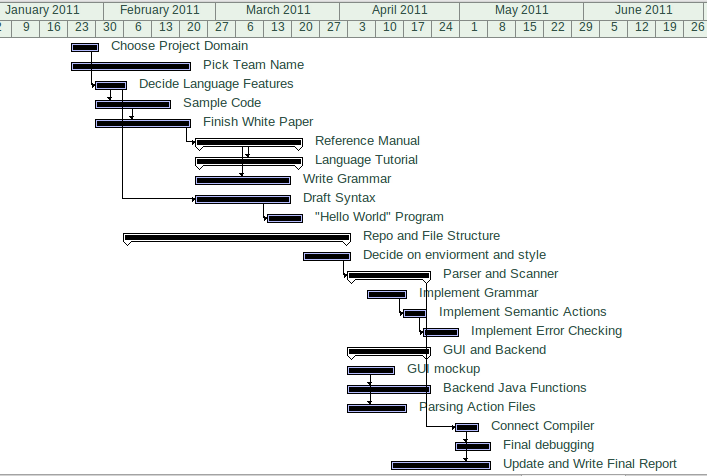
\includegraphics[scale=0.7]{project_timeline.png}

\section{Meeting Log}

\begin{flushleft}
\begin{singlespace}
\begin{tabular}{ | p{2cm} | p{1.8cm} | p{12cm} | }
\hline
\textbf{Meeting} & \textbf{Date} & \textbf{Minutes}\\
\hline
\textbf{1} & Jan 24th & Brainstormed ideas for programming language. An idea that was discussed: we give users the option of using simple statements to design say maybe a Rubik cube game with a high degree of customisation; not only can the sides of the cubes be coloured, we can leave it to the imagination of the users to say, maybe use texts on the smaller cubes and come up with a creative game involving the Rubik cube or say even a sphere.\\
\hline
\textbf{2} & Jan 26th & More ideas discussed: The  Programmer gets to upload the instrumental, type the lyrics in the code/upload the lyrics as well. They get to choose speed of highlighting for any given interval. The onus of syncing it with the corresponding part in the music is on the user. Another idea:  Just graphics and the ability to build complex games from shapes. You could have enough power to build tower defense, Angry Birds, Asteroids etc. without the fancy pictures. Just with pure shapes.\\
\hline
\textbf{3} & Jan 30th & Settled on some sort of Fantasy League Game. Some questions discussed: Is there a problem with connecting to the Database? What kind of data-types? Will it be object-oriented? How extensible should our language be? How should we design the syntax? Started draft of white paper.\\
\hline
\textbf{4} & Feb 6th & Continued Working on white-paper. Agreed that language should contain OO and be similar to Java but take elements from Python. Created Git Repo. Created team google-group.\\
\hline
\textbf{5} & Feb 9th & Agreed on Language Breakdown
A FLOOD program can:
\begin{itemize}
\item Create a league and define attributes such as team size.
\item Establish Rules for play using the existing libraries or overriding them.
\item Define features of the league such as draft and trade functions.
\item Connect the league to a database of the user's choice.
\item Trigger the build for the front end GUI and deploy the program to users.
\end{itemize}\\
\hline
\textbf{6} & Feb 13th & Continuing work on white-paper. Sketch of what a program would look like. Settled on possible name for project: FLOOD
First Commit to new repo.\\
\hline
\textbf{7} & Feb 17th & Discussing feedback from language brainstorming session.\\
\hline
\end{tabular}
\end{singlespace}
\end{flushleft}

\begin{flushleft}
\begin{singlespace}
\begin{tabular}{ | p{2cm} | p{1.8cm} | p{12cm} | }
\hline
\textbf{Meeting} & \textbf{Date} & \textbf{Minutes}\\
\hline
\textbf{8} & Feb 21th & Final Meeting to finish white-paper. Finalized language features and highlights, data-types, keywords and control-flow. Discussed possible application of a FLOOD program.\\
\hline
\textbf{9} & Feb 23rd & Submitted White Paper.\\
\hline
\textbf{10} & Mar 5th & Discussed Feedback from White-Paper. Where is our computation? How do we want to implement OO?\\
\hline
\textbf{11} & Mar 14th & All day session to work on RM and LT.\\
\hline
\textbf{12} & Mar 17th & All day session to work on RM and LT.\\
\hline
\textbf{13} & Mar 19th & Finishing the grammar, continuing the reference manual. Updated the Language Tutorial to reflect changes in grammar.\\
\hline
\textbf{14} & Mar 23rd & Submitted LT and RM.\\
\hline
\textbf{15} & Apr 3rd & Discussed ways to implement OO and whether to alter to the language and simplify it. Discuss times for final presentation.\\
\hline
\textbf{16} & Apr 8th & Feedback on LT and RM. Beginning to scale down the language to make it easier to write a parser and scanner.\\
\hline
\textbf{17} & Apr 10th & Project File Structure finalised and committed to repo. Division of labor and initial deadlines drawn up. First files committed to repo. Java and FLOOD files used for testing created. Meeting times for the rest of the project: Monday 6:15 pm, Thursday 6:15 pm. One weekend day to be chosen on Saturday 1:00 pm - Longer meeting to work (in CLIC lab).\\
\hline
\textbf{18} & Apr 11th & Revamped Syntax and started sketching GUI mockups.\\
\hline
\textbf{19} & Apr 14th & Working meeting in CLIC lab (see commit comments).\\
\hline
\textbf{20} & Apr 21th & Progress Report. Basic FLOOD file can be parsed.\\
\hline
\textbf{21} & Apr 26th & Working Meeting in CLIC lab (see commit comments).\\
\hline
\textbf{22} & Apr 28th & Working Meeting in CLIC lab (see commit comments).\\
\hline
\textbf{23} & May 2nd & Working Meeting in CLIC lab (see commit comments).\\
\hline
\textbf{24} & May 4th & Putting the final product together. Finished updating the reference manual and language tutorial. Error Checking in place. File FLOOD program can be compiled.\\
\hline
\textbf{25} & May 6th & Last minute debugging. Adding more error productions. Last run-through of every unit test with whole team present.\\
\hline
\textbf{26} & May 8th & Preparing Presentation. Looking over Final Report last time.\\
\hline
\end{tabular}
\end{singlespace}
\end{flushleft}


\chapter{Language Evolution (Anuj)}

At the onset of our language development, we decided to provide the user with as much flexibility as possible. With this as the main focus, our language was aimed at providing object-oriented development to the users. Bearing this in mind, we began developing our language in an incremental manner. We first decided on what the output of the front-end should be, based on what the back-end would expect. In short, we settled on the rendezvous point for the front-end and back-end and worked our way towards it.

As we deliberated on what this intermediate Java code should be, we realized it would be sufficient if the back-end is object-oriented. We therefore decided that the onus of object-oriented programming should not be on the programmer, keeping in mind that users of \textbf{FLOOD} will most likely not be familiar with object-oriented concepts. Moreover, we concluded that given the nature of the domain, the programming language being object-oriented would make the learning curve steeper for the user with not much added value. Fully convinced along these lines and the ease-of-use for the programmer in mind, we decided to do away with the object-oriented paradigm.
 
With the face of the language now modified to provide the user with as much flexibility as needed, yet within the domain of the language as well as keeping it simple to program, we set out to decide the logical division of the program code to aid the user in programming. We carefully analysed fantasy leagues and realized there exists a common denominator between all fantasy leagues. We decided to push this common denominator to the back-end, leaving the user with the bare minimum yet retain full flexibility to design a fantasy league with the rules of his/her choice.

The language now was developed with a logical division of the program the developer would have to write. The first would need to be the definition of the league; the programmer would need to specify details of the number of users, the names of the users, the players and their scores, valid actions and points associated with these valid actions. This allows the user to define rather quickly the parameters and setup the league.

The next logical block we decided on was defining functions and invoking them within other functions. This section needs to begin with the keyword \texttt{DefineFunction}. There are four default functions that each league needs to have which are: \texttt{draftPlayer}, \texttt{dropPlayer}, \texttt{trade}, \texttt{draftFunction}. The user can override these functions, although the user can choose not to define these functions, and the default function definitions for these functions will be invoked. 

Over and above these four functions, the user can define custom functions and invoke them. In its first incarnation, functions could take any number of parameters of the following types: \texttt{Bool}, \texttt{Str}, \texttt{Int}, \texttt{Flt}. Variable declarations were allowed at the beginning of the function before any other statements. The language at this point also provided looping structures, arithmetic expressions, relational expressions as well as conditionals. The back-end required array constructs of objects of a couple of back-end classes, namely the \texttt{User} and \texttt{Player} classes. Since the programmer does not know the contents of the \texttt{User} and \texttt{Player} classes, we decided to introduce array constructs in the formal parameters and actual parameter list of functions as follows:

\begin{alltt}\begin{singlespace}
         functionName(User[] u,Player[] p) \{ statements \}\end{singlespace}
\end{alltt}

In this manner, when changes were made in the grammar they were incorporated in the back-end and conversely, when changes were made to the back-end, they were incorporated in the grammar. The evolution of the language thus meant the grammar and the back-end evolving in tandem and incrementally.

\chapter{Language Architecture (Tam)}

The basic tools used to design the translator are \textbf{JFlex} for lexical tokenization and \textbf{BYACC/J} for the compiler generator. The lexical tokens are listed in the \textbf{JFlex} file, \textit{flood$\_$lex.flex}. \textbf{JFlex} tokenizes the input and passes the input in the form of these tokens to the parser, \textbf{BYACC/J}.

The grammar that the language follows is defined in the \textbf{BYACC/J} file, \textit{flood$\_$grammar.y}. Once this file is compiled, the generated Java file, \textit{Parser.java} is the parser generator for our language. The semantic actions to be performed on the input file given to our compiler are listed in the semantic action of each production in the \textit{flood$\_$grammar.y} file. These semantic actions involve type checking, arithmetic logic, function definitions and variable definitions. If any error is detected in the input file, our parser will not generate the output and will display the error. The high level view is illusrated in the following figure:

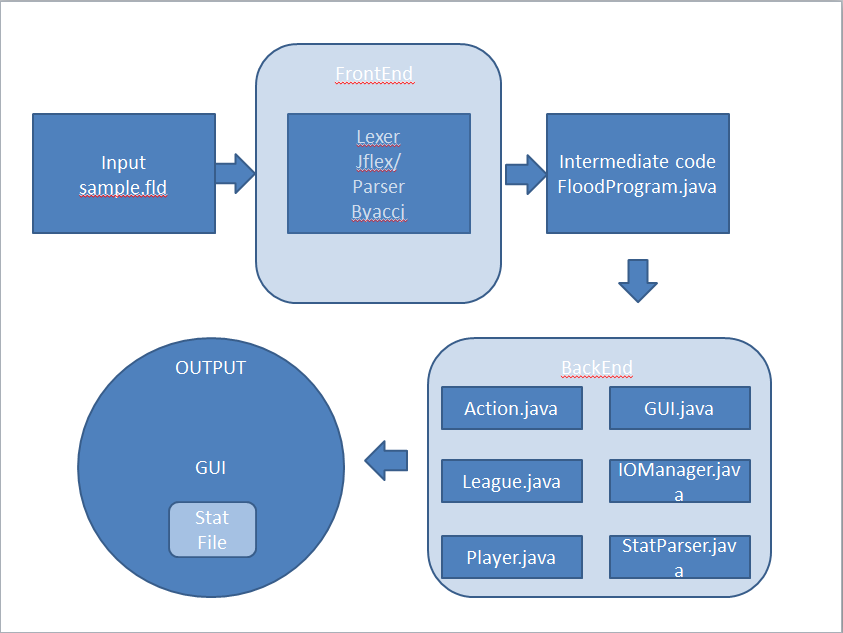
\includegraphics[scale=0.7]{system_architecture.png}

If the input is accepted by our strongly typed language, the front-end generates the intermediate code, \textit{FloodProgram.java}. On compilation and execution, the back-end generates the output in the form of a GUI.

The back-end of the system consists of all the Java files that the intermediate code references to generate the output. The GUI of the system makes use of a \textit{Statistics} file which holds the statistics of the proceedings of the league. Based on these statistics, the GUI generates the ranking of each user in the league which determines the winning user at any point.

\section{Module Authors}
\begin{singlespace}
\begin{itemize}
\item Grammar design and implementation : Tam and Anuj.
\item Semantic actions: Dillen, Stephanie and Elliot.
\item Backend: Dillen.
\end{itemize}
\end{singlespace}

\chapter{Development Enviornment (Dillen)}

During the development of the \textbf{FLOOD} language, development was spread across two operating systems. The majority of the group developed with \textbf{Ubuntu} (10.04/10.10/11.04) while one other worked exclusively in \textbf{Windows} 7 which ended up working out rather smoothly despite some issues setting up the \textbf{Git} repo on \textbf{Windows} and maintaining multiple \textit{makefiles}. Yet this cross system development also ensures that our language is not system dependent. In order to maintain a current version of all parts of the language, our group set up an online repository on \textbf{GitHub} where changes could be made at any time at the programmer's convenience.

The majority of Java code for the source files used in the intermediate code compilation level was written nearly exclusively in \textbf{Eclipse} 3.6 \textit{Helios}. The majority of the back-end was written from scratch with a select few data structures to promote efficiency. Those libraries included primarily the Java API's \texttt{HashMap} and \texttt{ArrayList} classes when necessary so that looking up references to various \textit{Users}, \textit{Players} and \textit{Actions} would all be $O(1)$. They were also used in a manner to prevent duplicate copies of any particular instance of class so that references (values of references since Java is pass-by-value) were used instead.

In addition to these source files, a GUI was also created to allow user interaction with the program during runtime, a key component of any fantasy league. The development of the GUI was restricted to purely Java's \textbf{Swing} and \textbf{AWT} library components with the framework created using Google's \textbf{WindowBuilder Pro} web toolkit. With the assistance of the development environment provided by that plugin to \textbf{Eclipse}, the GUI's rough layout was generated with ease but was completely devoid of any functionality besides its good looks.

The remainder of the GUI was developed by hand adding various functionalities to different components and promoting ease of integration with files generated by the compiler. No other outside sources were used in the remainder of the production of the source files that integrate with the compiler output besides the occasional Google search on how some feature of \textbf{Swing} truly worked, disregarding one's intuition. The final features added to the GUI were the ability for the program to write its current state to a file that could be saved in a directory and then imported at a later date, so that a fantasy league could be easily maintained over the course of any sports season without leaving a program running for the entire duration.

The parser and grammar were implemented with \textbf{JFlex} and \textbf{BYACC/J} respectively. These are both the Java versions of \textbf{Lex} and \textbf{Yacc} that the language \textbf{FLOOD} compiles to in its intermediate code generation. The majority of the development of the parser and grammar were done in a combination of \textbf{Gedit}, \textbf{TextPad}, terminal along with some good ol' fashioned paper and pencil. Paper and pencil is really the best (and almost only) way to really work out and recognize shift/reduce conflicts which inevitably helped to understand in general their origins and prevent them. The only exclusion to this trend was the development of the semantic actions that enforced type checking and other semantic checks, such as determining if functions and variables had been previously declared, which were primarily developed in \textbf{Eclipse} 3.6 \textit{Helios}. This was done due to the fact that it was exclusively written in Java in which instantaneous compilation helped with simple syntax errors that may have been overlooked.

The most important tool, however, used in the joint production of \textbf{FLOOD} was indubitably \textbf{Google Docs}. The ability to jointly work on the \textit{White Paper/Language Tutorial/Reference Manual} and watch them come together smoothly as opposed to very disjoint and extremely different written components was truly invaluable. The ability to share and jointly edit other's documents such as schedules, bug reports and other files simultaneously without the burden of constantly pulling and pushing vastly improved efficiency especially when every group member can just consult a checklist to see what components were still incomplete and most urgent. Additionally, the real time updating of files provided a great base for the conversion to \textbf{\LaTeX} of the final reports. It was a crucial component in the merging of everyone's work throughout the process.

\chapter{Test Plan (Stephanie)}

In the early stages of developing the grammar for \textbf{FLOOD} most testing simply followed this scheme:

\begin{itemize}
\item Write a line of code.
\item Test it.
\item Does it work?
\begin{itemize}
\item Yes
\begin{itemize}
\item Jump to first statement.
\end{itemize}
\item No
\begin{itemize}
\item Rewrite line of code.
\item Jump to second statement.
\end{itemize}
\end{itemize}
\end{itemize}

This practice was less about writing production code, and more just to explore and understand \textbf{Lex} and \textbf{Yacc}.

Soon, the grammar began to take shape. As we developed the expressions and loops, fuller and more thorough unit test programs needed to be generated. As each complete production was a made, at least two accompanying unit test programs were written to test that production. The two unit tests would test for correctness as well as for failure, meaning that one unit test was meant to be successful, while the other was meant to fail. Often there was more than one unit test intended to fail, because there are multiple ways in which any single part of the program could fail.

Once the grammar reached a self sustainable level, semantic checks began to be implemented. This checks would cover errors that the grammar could not handles on its own. The testing therefore, became more rigorous in order to cover all possible bases. At this point, unit testing included the full team in order to be as thorough as possible. As each member wrote semantic checks or edited the grammar they were encouraged to think of unit tests to break whatever they just wrote. These tests would be written and compiled together as they applied to each specific part of the language, and tested against the compiler. As it became increasingly more difficult to come up with unit tests, we would move on to the next semantic check, determining that the current tests sufficiently checked all possible error and success cases.

\section{Example Unit Tests}

\subsection{Unit Test 1}

\begin{singlespace}
\begin{lstlisting}[language=Java,label=some-code,caption={arithmetic$\_$test.fld}]
DefineLeague
	Set LeagueName("Happy League");
	Set MaxUser(10);
	Set MinUser(12);
	Add User("Eli");
	Add Action("Field Goal Attempt", 0.5);

DefineFunctions
	Int myFunction(Int turn, Flt turn2)
	{
		Str a;
		Str c;
		Str d;
		Bool b = True;

		a = a + c + d;		
		Return a;
	}
\end{lstlisting}
\end{singlespace}

The above unit test was meant to test the concatenation of strings. It is a functioning simple \textbf{FLOOD} program.

Below is one of it's counterparts. This program is meant to fail because it tries to add a boolean to the strings.

\begin{singlespace}
\begin{lstlisting}[language=Java,label=some-code,caption={arithmetic$\_$test.fld}]
DefineLeague
	Set LeagueName("Happy League");
	Set MaxUser(10);
	Set MinUser(12);
	Add User("Eli");
	Add Action("Field Goal Attempt", 0.5);

DefineFunctions
	Int myFunction(Int turn, Flt turn2)
	{
		Str a;
		Str c;
		Str d;
		Bool b = True;

		a = a + c + b;		
		Return a;
	}
\end{lstlisting}
\end{singlespace}

\subsection{Unit Test 2}

\begin{singlespace}
\begin{lstlisting}[language=Java,label=some-code,caption={array$\_$var$\_$index.fld}]
DefineLeague
	Set LeagueName("Happy League");
	Set MaxUser(10);
	Set MinUser(12);
	Add User("Eli");
	Add Action("Field Goal Attempt", 0.5);

DefineFunctions
	Bool random(Player p1)
	{
		Bool b;
		b = True;
		Return b;
	}

	Bool trade(User u1,Player[] p1, User u2, Player[] p2)
	{
		Int i = 1;
		Bool b;
		b = random(p1[i]);
	}
\end{lstlisting}
\end{singlespace}

The above unit test is meant to check user defined functions as well as array indexing. Two of its counterparts are shown below. The first fails because the function is defined after it is called.

\begin{singlespace}
\begin{lstlisting}[language=Java,label=some-code,caption={array$\_$var$\_$index.fld}]
DefineLeague
	Set LeagueName("Happy League");
	Set MaxUser(10);
	Set MinUser(12);
	Add User("Eli");
	Add Action("Field Goal Attempt", 0.5);

DefineFunctions
	Bool trade(User u1,Player[] p1, User u2, Player[] p2)
	{
		Int i = 1;
		Bool b;
		b = random(p1[b]);
	}

	Bool random(Player p1)
	{
		Bool b;
		b = True;
		Return b;
	}
\end{lstlisting}
\end{singlespace}

The second fails because it attempts to use a boolean as the index of an array.

\begin{singlespace}
\begin{lstlisting}[language=Java,label=some-code,caption={array$\_$var$\_$index.fld}]
DefineLeague
	Set LeagueName("Happy League");
	Set MaxUser(10);
	Set MinUser(12);
	Add User("Eli");
	Add Action("Field Goal Attempt", 0.5);

DefineFunctions
	Bool random(Player p1)
	{
		Bool b;
		b = True;
		Return b;
	}

	Bool trade(User u1,Player[] p1, User u2, Player[] p2)
	{
		Int i = 1;
		Bool b;
		b = random(p1[b]);
	}
\end{lstlisting}
\end{singlespace}

\chapter{Conclusions}

\section{Lessons Learned as a Team}

We feel that as a team we have a better understanding of the magnitude of large programming projects. We learned that initial ideas are seldom translated into the final product. When the project first began, we had intended to write a very large language with many features. At the time, none of us truly understood the work that went into implementing even a small language. As we progressed in the semester, the difficulty of the task became more apparent and we had to change our entire language. We feel that we learned a great deal about the more complex aspects of programming languages specifically because we were not able to implement what we had originally intended. Trying to brainstorm features like inheritance and polymorphism taught us about how those components work in popular programming languages. 

We learned that teamwork doesn't mean everyone does their own part. It means that people help out and don't stay contained within their respective responsibilities. It means that if someone is having an off-week and/or has an exam the next day, other team members can carry the weight that meeting. We learned that work-schedules need to be implemented early and ambitiously so that deadlines can be stretched within reason if needed.

We each learned different ideas on programming and development from our teammates. Every session of programming there were arguments of proper programming practices or the design of the language. Team members contributed ideas to our language from a wealth of programming experience from languages such as Java, C++, Python and Pascal. We learned that that every team member has particular strengths and those should be utilized as often as possible.

\section{Lessons Learned by Each Team Member}

\subsection{Stephanie}

\begin{enumerate}
\item The greatest lesson I learned from this assignment was to \textit{start small and work your way up from there}. Designing a project that implements something you have no idea how to do is extremely difficult. It is all too easy to fall into a very complicated design when the process for creating the pieces is not yet known. In the beginning, my team and I were rather ambitious and naively so. We had dreams of an object-oriented language complete with inheritance, polymorphism, and encapsulation. We even wanted to expand the language onto the \textbf{Android} platform if we had time. Somehow we had forgotten what college was: four years of spending every minute of every hour wishing you had more time. We soon realized the we were in way over our heads, and that there was only so much weight Java would carry for us. And so, we had to significantly modify our approach to this project. We first started by simply making cuts to the language, but that left a convoluted and disorganized language. So instead we began anew. We identified all the bare minimum requirements needed for a fully functional language for generating fantasy leagues. From there we could build a base language and then add to that. This process takes away depressing decisions to remove ideas, and replaces it with the exciting realization that we can add things.
\item \textit{Projects of this magnitude need to be constantly worked on}. You can't simply wait until a week before a deadline, put in endless hours of work and expect that to be sufficient. When a project spans four months work must be put into it every week of every month. By getting into lulls where no work is being done on the language, you risk losing focus and generating a bit of a learning curve, if you will, in order to return to the language. Right from the beginning, we made sure to meet regularly, regardless of how much we needed to do. There needed to, at the very least, be a constant reminder of the project, no time for the language to be forgotten.
\item While at times it may appear to be rather difficult, it is important to \textit{always be aware of what each team member is working on}. Not in the sense that you know specifically what they are doing every minute they are working, but just where they are. Indeed, that is primarily the job of the project manager, but I found that it is rather helpful for each member of the team to communicate with the team what their next steps were and how they were going to go about completing their goals. This way there is minimal disconnect between the various parts of the language, especially between semantics and the grammar, where changes in one greatly affect the other. Our group maintained this awareness with the use of \textbf{GitHub}, \textbf{Google Docs}, and a \textbf{Google Group}, in addition to our frequent team meetings and coding sessions. This way, all changes were documented and spread throughout the entire group.
\item \textit{The project is a not a group of people designing pieces of a puzzle that will fit together, after quite a bit of massaging and molding, to produced a result}. It is a team building block after block, each block being guided onto the last, until the structure is complete. The idea to split the group into 5 specific roles helps with ensuring that everyone has a part to do, however I find that this can actually create a disconnect. Instead of creating a strict line on who does what, I feel that having each person contribute to each part of the language builds a more continuous final product. Moreover, it makes the process of merging the parts of the language significantly more efficient because each member of the teams understands the language and many errors are avoided or resolved quickly by simply just knowing what to look for. In summary it creates a cohesive team, with a thorough understanding of the language.
\item \textit{Commitment is a vital key to any successful team project}, and for a project that has lasted as long as this, it is all too easy to feel overwhelmed. Over the course of the semester fluctuations in one's workload and personal life can take quite a toll on one's ability to function in a group. However, it is in these times that the true power of the group shines through. In the first couple weeks after I fractured my hand, the pain was enough to inhibit my ability to type. In that same time, I had a web site to build, an essay to write, and coding sessions for this project. Had it not been for my team, I would have likely given in to the stress and crumpled under the workload. However, my determination to not let my teammates down allowed me to continue pushing forward. This level of commitment can develop in a team regardless of whether or not the team member knew each other before the formation of the team. When the members of \textbf{FLOOD} were established, I only knew half of my teammates. However, in a team of only 5, it is hard to remain cliquish and as a result the team developed rather strongly. Throughout the course, I've have become rather close friends with my team members and will look forward to taking classes with them in the future.
\end{enumerate}

\subsection{Elliot}

While this is not my first time as a project leader, it is my first time leading a software development project. The most important lesson I've learned is the need for constant communication among the team. At times though not often, information would be bottle-necked to a certain person and other team members would not be informed of important changes. The best way to deal with this situation is transparent documentation and meetings. I've also learned how difficult it can be for each team member's unique coding and work style to be integrated into a cohesive unit. For instance, our version control choice was unfamiliar to some team members at first and it took some time for everyone to get used to working with it.

A project of this magnitude can easily overwhelm any group no matter how experienced. The main goal should be constant pressure. Constant pressure does not mean stress but rather always making progress regardless of the difficulty or clarity of the task. Tasks should be constantly broken down into smaller pieces and distributed as evenly as possible. When a task is assigned, it shouldn't be assumed that the team member will be able to complete it but rather teammates should look out for each other and help when needed. The role of a product manager is not to dictate and assign tasks as they please. Every team member should be given the opportunity to pick specific tasks that they find most interesting. Tasks that were deemed uninteresting were distributed evenly so that no one took more than their fair share of ``grunt" work. Decisions should not only be democratic but accepted by the whole team. If even one team member didn’t like an idea or an implementation detail, the team worked hard to come up with an alternative that was acceptable to everyone. A product manager should also keep accurate records and have awareness of every moving piece in the project. Ultimately, as the saying goes, the ``The Buck Stops Here." This is a lesson every good product manager must learn and usually the hard way.

On a personal note, I feel comfortable saying I understand how a compiler works on a very applied level. I still don't feel comfortable with much of the theory that goes into compilers and in a way it has given me a healthy respect for theorists who have paved the way for modern programming languages. I learned to appreciate the intricacies of programming languages and notice subtle differences that were not obvious to me beforehand. I have already seen a difference in my code production in other projects. In my opinion, one of the most fascinating aspects of software development is the relationship among the developers. Working with other people, especially in an academic setting, is always challenging but it can also be very rewarding. I truly enjoyed the time spent working with my teammates and regardless of the final outcome of this project or the class in general, I feel that I have learned a great deal from them.

\subsection{Tam}

Ah, the project post mortem. Having recently worked in industry, I have personally been an active (and at times, unwilling) participant of countless such ``taking stock" couch sessions. More often than not, and especially after a grueling projects which taxed the mind and body as well as the soul, my own thoughts inevitably turned towards alcohol---nothing like dousing the brain cells which served me so well during those sleepless nights of feverish coding!

But after the welcome, and hopefully pre-paid, happy hour courtesy of a sympathetic Project Manager, gathering one's thoughts and indeed ``taking stock" to formulate a list of lessons learned is an invaluable exercise, one which will yield far-reaching benefits down the line for both developers and project managers alike.

At this stage of the game, I find myself asking a similar set of questions:

\begin{enumerate}
\item \textbf{First and foremost, are you proud of the final product?}\\
I will not be so presumptuous as to answer for my fellow group members, but I can say without hesitation that yes, I am very proud of \textbf{FLOOD}. Admittedly, certain features and overall scope were made road kill on the highway to making delivery, but such are the vagaries of software development. In fact, I now recall with particular fondness our formative group meetings in which, undoubtedly pie-in-the-sky-ish in retrospect, we brainstormed and flung around countless ideas about what our language will be capable of once completed. An Android-enabled interface! A Facebook port! Automatic texting of scores and live updates to subscribed listeners! Object-orientation that will make Java blush!\\
Not surprisingly, the majority of these ``nice to haves" fell by the wayside as the project progressed, but did we as a group accomplish what we set out to do originally, which was to write a language that made creating a fantasy gaming league relatively easy for the programming novice? I would say the answer is a resounding \textit{YES!}\\
And in undertaking this project, did I myself take away what is perhaps the most crucial aspect of completing the project and taking this class in the first place, which was to gain and learn from first-hand experience the inner workings of compilers and programming languages? Again, an uniequivocal \textit{YES!} Lexical analysis, semantic analysis and actions, code generation and optimization...nothing like rolling up one's sleeves and learning these concepts the hardway: by actually doing it.
\item \textbf{What was the single most frustrating part of the project?}\\
Hands down, tackling the lexical and semantic analysis of the grammar. Hours upon hours consummed in devising regular expressions that would do what we wanted it to do, then tracking down and eliminating with extreme prejudice countless shift/reduce reduce/reduce errors. With my comrade in arms, Anuj, the two of us now feel like battle-hardened veterans returning from the front-line trenches in our seemingly neverending battle against the Lexical/Semantic axis of power.\\
Did \textbf{FLOOD}'s grammar put up a valiant fight? Yes. Was it frustating to slay this merciless dragon? Yup...Anuj and I certainly have the mental scars to show for it. But in the end, was it rewarding? Most definitely. I have been involved in few software development projects where the most frustrating part was also the most personally fulfilling. This was one of them.
\item \textbf{How would you do things differently next time to avoid this frustration?}\\
Start learning the concepts and obtaining the knowledge one will need as early in the project timeline as possible. I believe my biggest mistake was taking such a timid approach towards the grammar---instead of waiting for the material to be presented and covered in class, we (I'm certain Anuj would agree) should have been more pro-active in acquiring the know-how and skill sets needed to write \textbf{FLOOD}'s grammar. And speaking for myself once more, there was also an intimidation factor at play since the tools for creating the front-end components of a compiler seemed truly daunting to me to work with. It's difficult at times teaching an old dog new tricks.
\item \textbf{What was the most gratifying and personally satisfying part of the project?}\\
This old dog learned a new trick. I didn't know how to write a lexical parser and scanner before. Now I do.
\item \textbf{Which of the development methods or processes worked particularly well?}\\
The pair programming Anuj and I undertook in developing the grammar. Over time we developed a comfortable working style that proved to be most productive. I was skeptical at first regarding this programming paradigm since nearly all of my industry experience has been working and coding in isolation, but engaging in pair progamming for the very first time was a truly eye-opening experience. Where before I would run into a dead-end in some coding dark alley, Anuj was often there to shine a flash light and lead the way out.
\item \textbf{If you could wave a magic wand and change anything about the project, what would you change?}\\
More time with my fellow \textbf{FLOOD}-ites. I was very blessed to have lucked into this group of highly motivated, extremely hard working, and very intelligent individuals. Sure, there were disagreements, some heated discussions, the occasional philosophical differences, but in the end we had a blast working together to give birth to \textbf{FLOOD}. I wish all of my future (and certainly several past) collaborative efforts will be as enjoyable and mutually beneficial as this one. I learned a great deal from my team and I hope I have reciprocated in kind---a true highlight of my academic career at Columbia.
\end{enumerate}

\subsection{Dillen}

\begin{enumerate}
\item \textbf{Choose your group members wisely.}\\
Choosing the right people for a group is beyond the most important part of an assignment. Although it may seem unclear what everyone's exact roles may be for a given project, be sure to pick people who are passionate and have deep interest in different components as well as the overall idea of a project. Nothing can be more detrimental to a group that to have members who are unenthusiastic or not willing to pull their own weight, not due to a lack of ability (because let's be honest, no one knew how a compiler worked when we first started) but rather a lack of motivation. Our group functioned extremely well because we all split up the parts into relatively equal work loads and when one part ``overflowed" due to unforeseen complexities, those with ``easier" tasks jumped in to help. Another key part of our success was the general interest in our idea, which became my next lesson learned.
\item \textbf{Thoroughly develop your idea, and then do it again.}\\
It is important to spend adequate time to thoroughly develop an idea and delve past the surface challenges and really research potential dead-ends. Unlike most groups (I believe), we met every week from the moment our group was formed until the end of the semester, even when we all lacked any detailed view of how to complete the task. The first several meeting were literally $4+$ hour long discussions on potential programming languages where everyone would express interest, play devil's advocate and expand on ideas. The most difficult part for us was to propose ideas feasible for a semester long project without simply creating a markup language. This was crucial in creating a thorough blueprint for our language and the writing of the \textit{White Paper/Language Tutorial/Reference Manual}.
\item \textbf{Don't reinvent the wheel.}\\
One of the most valuable parts of any programming project is to utilize tools provided online to ease the pain. Development tools such as \textbf{WindowBuilder Pro} for the GUI, \textbf{BYACC/J} and \textbf{JFlex} for the grammar and parser, \textbf{GitHub} for the online repository and \textbf{Google Docs} for the written portions provided greater ease and efficiency during the entire process. \textit{USE THEM!}
\item \textbf{Pick a good project manager who can bring everyone together.}\\
It is easy to get lost in time when everyone is specializing on a specific part of a project and it's the product manager's job to keep bringing everyone together and making sure everything is running smoothly and no individual is lagging behind. Collaboration and communication are absolutely key in the software development world because otherwise, come submission time, everyone has a bunch of extremely well developed but independent portions of the project with integration being nearly impossible. I noticed that our group was exceptionally productive when we all worked in one long line in the CLIC lab, each with the \textit{Google Bug Report Document} constantly asking questions, finding bugs and delegating work with various priority. I realize it is difficult for a bunch of college students to find time to all meet and work for a few hours but those hours spent working together are far more valuable than any work you will do by yourself.
\end{enumerate}

\subsection{Anuj}

\begin{enumerate}
\item \textbf{Grammar design is not a walk in the park.}\\
Designing the grammar for a language is not easy. Designing a small grammar for small units, like say, just arithmetic expressions, is easy. As the grammar evolves, the complexity increases linearly. It helps to have a clear idea of what the language will look like and stub out a rough design of the grammar first. This methodoloy exposes the potential shift/reduce and reduce/reduce errors right from the beginning. It also helps to understand fully how these errors occur and how to eliminate them.
\item \textbf{Decide the scope of the language/project realistically.}\\
One of the most important lessons I learned from this project is to do a strong feasibility study before proposing a project. A thorough study should be performed to roughly estimate what problem statement the project proposes to tackle. It should neither be too ambitious nor too trivial. Getting the right balance is a tricky task and it seems safer to project the latter and extend the scope of the project if time permits. Another important lesson I learned is never to commit any major feature in the name of the project unless absolutely certain that the feature will be implemented!
\item \textbf{Working in a group.}\\
To begin with, I had an interesting time working with my group. It not only made working on a project of this magnitude seem effortless, but I also learned a lot from my group on various fronts. This made me realise how important team members are and the dynamics of the group can make or break a project. While it may seem more hands on deck means less work per person, I also realised it requires good management on the part of the Project Manager to coordinate and integrate the project well; something I was privy to during the course of this project.
\end{enumerate}

\section{Advice for Future Teams}

\begin{itemize}
\item \textit{\textbf{Never}} promise features of your programming language in its name. We tried very hard to come up with a ``cool" name that described our language. The name is still ``cool" but it doesn't describe our language anymore.
\item Start early and meet often. It may seem futile to meet when you have nothing to discuss but just by being in the same room you may start thinking of an idea that changes your project.
\item Ask for help no matter how small of an issue. We utilized our TA, Hemanth, as much as possible and we are truly indebted to him for all his valuable advice.
\item Don't be scared of unfamiliar technology; free software is your friend. Our entire project was written and shared in \textbf{Google Docs}, the code will forever be saved on \textbf{GitHub} and the documentation lives beautifully in \textbf{\LaTeX}.
\item Revisit your idea as much as possible. Our language has morphed from an object-oriented language with Java-like features into a smaller, more compact version. If we had decided to go ahead with our original idea we would not have finished our project or it would have been poorly implemented.
\item Pair programming may seem like a waste of time but it dramatically reduces net production time. Most of the code produced was written at one work station with two team members working at a time. Often code that seemed very difficult to one programmer was trivial to another. When a programmer was tired, they could switch and development continued.
\item Pick a project that is interesting to you rather than trying to impress anyone. Every team member was truly interested in our project which made brainstorming more fun and productive. 
\item A team that eats together works better. It's better to work on a full stomach and it's more fun to brainstorm over dinner. We personally recommend the Dominoes 7-7-7 deal.
\end{itemize}

\section{Suggestions for Future Improvement}

It's very difficult to write this section as a team since each team member had different topics that they enjoyed. We all agree that the project was the highlight of the course and very much enjoyed working on it. Some of us feel that the classes were a little theory-heavy in what was originally expected to be a more applied course in compilers. Some of the theory, especially the later topics such as code-generation and optimization as well as data-flow analysis might have been better served with more homework and possibly programming exercises.

The first homework gave everyone a taste of \textbf{Flex} and \textbf{Yacc} which helped both in understanding the theory and what was expected later in the project. Those of us who had taken \textit{Computer Science Theory} enjoyed seeing how the theory we had previously learned applied in the ``real-world." We all feel that this was a difficult class but in the end truly rewarding.

\appendix
\chapter{FLOOD Source Code}

\begin{singlespace}
\begin{lstlisting}[language=Java,label=some-code,caption={Action.java}]
/*
 * Action.java
 * This class handles the various actions in the fantasy league
 */

public class Action {
	private String action;
	private float points;
	
	/**Constructor.
	 * 
	 * @param String action
	 * @param float points
	 */
	public Action(String action,double points){
		this.action=action;
		this.points=(float)points;
	}
	
	/**Returns the string representation of the action
	 * 
	 * @return String action
	 */
	public String getAction() {
		return action;
	}
	
	/**Sets the action
	 * 
	 * @param String action
	 */
	public void setAction(String action) {
		this.action = action;
	}
	
	/**Return the points gained for completing the action
	 * 
	 * @return float points
	 */
	public float getPoints() {
		return points;
	}
	
	/**Sets the points gained for completing the action
	 * 
	 * @param float points
	 */
	public void setPoints(int points) {
		this.points = points;
	}
	
	/**Determines if two actions are equal by comparing
	 * the action and points received
	 * 
	 * @return boolean isEqual
	 */
	public boolean equals(Object obj){
		if (this == obj)	//Reference to seld
			return true;
		if (obj == null)	//Null reference
			return false;
		if (getClass() != obj.getClass())	//Not the same class
			return false;
		final Action other = (Action) obj;
		if (action.equals(other.action) && points==other.points)	//Equal action and points
			return true;
		return false;
	}
	
	/**Returns a string representation of the action
	 * 
	 * @return String representation
	 */
	public String toString() {
		return "Action [action=" + action + ", points=" + points + "]";
	}
	
}
\end{lstlisting}
\end{singlespace}

\begin{singlespace}
\begin{lstlisting}[language=Java,label=some-code,caption={flood$\_$grammar.y}]
/* * * * * * * * * * * * * * * * * * * * * * * * * * * * * * *
*
* flood_grammar.y
* FLOOD
* Syntactic/Semantic Analyzer
* Lasciate ogne speranza, voi ch'intrate
*
* * * * * * * * * * * * * * * * * * * * * * * * * * * * * * */

%{
  import java.lang.Math;
  import java.io.*;
  import java.util.Hashtable;
  import java.util.ArrayList;
  import java.util.Iterator;
  import java.util.HashMap;
  import java.util.*;
%}

/* YACC Declarations */
%token PLUS                   /* + */
%token OPEN_CURLY             /* { */ 
%token CLOSE_CURLY            /* } */
%token OPEN_PARAN             /* ( */
%token CLOSE_PARAN            /* ) */
%token OPEN_SQUARE            /* [ */
%token CLOSE_SQUARE           /* ] */
%token <dval> FLT             /* Float */
%token <ival> INT             /* Integer */
%token <sval> STRING_CONST    /* String literal onstants */
%token COMMA                  /* , */
%token DOT                    /* . */
%token <sval> ID              /* Identifier */
%token EQUAL                  /* = */
%token NOTEQUAL               /* != */
%token LESSEQUAL              /* <= */
%token GREATEQUAL             /* >= */
%token ISEQUAL                /* == */
%token LESS                   /* < */
%token GREAT                  /* > */
%token PLUS                   /* + */
%token MINUS                  /* - */
%token MULT                   /* * */
%token DIV                    /* / */
%token NOT                    /* ! */
%token AND                    /* && */
%token OR                     /* || */
%token MOD                    /* % */
%token SEMICOLON              /* ; */

/* Keywords */
%token DefineLeague           /* Define the league */
%token DefineFunctions        /* Define functions */
%token LeagueName             /* Set league name */
%token MaxUser                /* Set the max user */
%token MinUser                /* Set the min user */
%token MaxTeamSize            /* Set the max team size */
%token MinTeamSize            /* Set the min team size */
%token Set                    /* Set keyword */
%token Add                    /* Add keyword */
%token Action                 /* Action keyword */
%token Alert		      /* Alert message*/
%token Error		      /* Error message*/
%token User                   /* User keyword */
%token Player                 /* Player keyword */
%token Void                   /* Void keyword */
%token Str                    /* String keyword */
%token Bool                   /* Boolean keyword */
%token Flt                    /* Float keyword */
%token Int                    /* Integer keyword */
%token Return                 /* Return keyword */
%token If                     /* If keyword */
%token Else                   /* Else keyword */
%token While                  /* While keyword */
%token True                   /* True keyword */
%token False                  /* False keyword */
%token RemovePlayer           /* Remove Player function */
%token AddPlayer              /* Add Player function */
%token ArrayLength            /* Length of an array */
%token GetUserName	      /* Gets the name of the user object*/
%token GetNumPlayers          /* Gets the number of players of the user*/
%token GetPlayerName          /* gets the name of the player object*/
%token GetPlayerPosition      /* Gets the position of the player*/
%token GetPlayerPoints        /* Gets the points of the player*/

/* Associativity and Precedence */
%left MINUS PLUS COMMA
%left MULT DIV
%right NOT NEG
%nonassoc EQUAL NOTEQUAL LESSEQUAL GREATEQUAL ISEQUAL LESS GREAT AND OR MOD DOT

/* Types */
%type <sval> definitions
%type <sval> definitionlist
%type <sval> definitionproductions
%type <sval> functions
%type <sval> functionProductions
%type <sval> returnType
%type <sval> dataType
%type <sval> functionName
%type <sval> argumentLists
%type <sval> argumentList
%type <sval> empty;
%type <sval> returnProduction
%type <sval> returnProd
%type <sval> statement
%type <sval> statements
%type <sval> conditionals
%type <sval> loop
%type <sval> declarations
%type <sval> declaration
%type <sval> relationalExp
%type <sval> arithmeticExp
%type <sval> booleanExp
%type <sval> constOrVar
%type <sval> leftSide
%type <sval> rightSide
%type <sval> assignment
%type <sval> functionCall
%type <sval> parameterList

%%

/***************************************************
* program
****************************************************/
program: definitions functions
{
	if(semantics.validProgram)
	{
		generateFloodProgram($1, $2);
		System.out.println("Total number of lines in the input: " + (yyline - 1));
	}
	else
	{
		System.out.println(semantics.printErrors());
	}
};

definitions: DefineLeague definitionlist { $$ = $2; };
           
definitionlist: definitionlist definitionproductions { $$ = $1 + $2; }
              | empty { $$ = $1; }
              ;

definitionproductions: Set LeagueName OPEN_PARAN STRING_CONST CLOSE_PARAN SEMICOLON { $$ = "myLeague = new League(" + $4 + ");\n"; }
                     | Set MaxUser OPEN_PARAN INT CLOSE_PARAN SEMICOLON { $$ = "myLeague.setMaxUser(" + $4 + ");\n"; }
                     | Set MinUser OPEN_PARAN INT CLOSE_PARAN SEMICOLON { $$ = "myLeague.setMinUser(" + $4 + ");\n"; }
                     | Set MaxTeamSize OPEN_PARAN INT CLOSE_PARAN SEMICOLON { $$ = "myLeague.setMaxTeamSize(" + $4 + ");\n"; }
                     | Set MinTeamSize OPEN_PARAN INT CLOSE_PARAN SEMICOLON { $$ = "myLeague.setMinTeamSize(" + $4 + ");\n"; }
                     | Add User OPEN_PARAN STRING_CONST CLOSE_PARAN SEMICOLON { $$ = "myLeague.addUser(new User(" + $4 + "));\n"; semantics.addUser($4, yyline); }
                     | Add Action OPEN_PARAN STRING_CONST COMMA FLT CLOSE_PARAN SEMICOLON { $$ = "myLeague.addAction(new Action(" + $4 + ", " + $6 + "));\n"; semantics.addAction($4, yyline); }
		     | Add Action OPEN_PARAN STRING_CONST COMMA MINUS FLT CLOSE_PARAN SEMICOLON %prec NEG { $$ = "myLeague.addAction(new Action(" + $4 + ", -" + $7 + "));\n"; semantics.addAction($4, yyline); }
                     | Add Player OPEN_PARAN STRING_CONST COMMA STRING_CONST CLOSE_PARAN SEMICOLON { $$ = "myLeague.addPlayer(new Player(" + $4 + ", " + $6 + "));\n"; semantics.addPlayer($4, yyline); }
                     ;

functions: DefineFunctions functionProductions { $$ = $2 + semantics.setFlags(); };

functionProductions: functionProductions returnType functionName OPEN_PARAN argumentLists CLOSE_PARAN OPEN_CURLY  declarations statements returnProduction CLOSE_CURLY { $$ = $1 +"public static "+ $2 + " " + $3 + "(" + $5 + ")\n{\n" + $8 + $9 + $10 + "\n}\n"; this.scope = $3; semantics.addToFunctionTable($3, $2, $5, yyline); semantics.checkReturnTypeMatch($2, yyline); }
                     | functionProductions returnType functionName OPEN_PARAN argumentLists CLOSE_PARAN OPEN_CURLY empty CLOSE_CURLY {$$ = $1 +"public static "+ $2 + " " + $3 + "(" + $5 + ")\n{\n}\n"; this.scope = $3; semantics.addToFunctionTable($3, $2, $5, yyline); semantics.checkReturnTypeMatch($2, yyline); }
                     | functionProductions returnType functionName OPEN_PARAN argumentLists CLOSE_PARAN OPEN_CURLY  empty statements returnProduction CLOSE_CURLY {$$ = $1 +"public static "+ $2 + " " + $3 + "(" + $5 + ")\n{\n" + $8 + $9 + $10 + "\n}\n"; this.scope = $3; semantics.addToFunctionTable($3, $2, $5, yyline); semantics.checkReturnTypeMatch($2, yyline); }
                     | functionProductions returnType functionName OPEN_PARAN argumentLists CLOSE_PARAN OPEN_CURLY  declarations empty returnProduction CLOSE_CURLY {$$ = $1 +"public static "+ $2 + " " + $3 + "(" + $5 + ")\n{\n" + $8 + $9 + $10 + "\n}\n"; this.scope = $3; semantics.addToFunctionTable($3, $2, $5, yyline); semantics.checkReturnTypeMatch($2, yyline); }
                     | functionProductions returnType functionName OPEN_PARAN argumentLists CLOSE_PARAN OPEN_CURLY returnProd CLOSE_CURLY {$$ = $1 +"public static "+ $2 + " " + $3 + "(" + $5 + ")\n{\n" + $8 + "\n}\n"; this.scope = $3; semantics.addToFunctionTable($3, $2, $5, yyline); semantics.checkReturnTypeMatch($2, yyline); }
                     | empty { $$ = $1; }
                     ;

dataType: Str { $$ = "String"; }
        | Bool { $$ = "boolean"; }
        | Int { $$ = "int"; }
        | Flt { $$ = "float"; }
        ;

returnType: Void { $$ = "void"; }
          | Str { $$ = "String"; }
          | Bool { $$ = "boolean"; }
          | Int { $$ = "int"; }
          | Flt { $$ = "float"; }
          ;
          
functionName: ID { $$ = $1; };

argumentLists: argumentLists COMMA argumentList { $$ = $1 + ", " + $3; }
              | argumentList { $$ = $1;}
              | empty { $$ = $1; }
              ;

argumentList: dataType ID { $$ = $1 + " " + $2; semantics.addVar($2,$1,yyline); }
            | User OPEN_SQUARE CLOSE_SQUARE ID { $$ = "User[] " + $4; semantics.addVar($4,"User[]",yyline); }
            | Player OPEN_SQUARE CLOSE_SQUARE ID { $$ = "Player[] " + $4; semantics.addVar($4,"Player[]",yyline); }
            | User ID { $$ = "User " + $2; semantics.addVar($2,"User",yyline); }
            | Player ID { $$ = "Player " + $2; semantics.addVar($2,"Player",yyline); }
            ;

statements: statements statement SEMICOLON { $$ = $1 + $2; }
          | statement SEMICOLON { $$ = $1; }
          ;

statement: conditionals { $$ = $1; }
         | loop { $$ = $1; }
         | relationalExp { $$ = $1; }
         | assignment { $$ = $1; }
         | functionCall { $$ = $1 + ";\n"; }
         ;

returnProduction: Return ID SEMICOLON { $$ = "return " + $2 + ";"; semantics.setReturnProdType(semantics.getType($2)); }
                | Return STRING_CONST SEMICOLON { $$ = "return " + $2 + ";"; semantics.setReturnProdType("String"); }
                | Return INT SEMICOLON { $$ = "return " + $2 + ";"; semantics.setReturnProdType("int"); }
                | Return FLT SEMICOLON { $$ = "return " + $2 + ";"; semantics.setReturnProdType("float"); }
                | Return True SEMICOLON { $$ = "return true;"; semantics.setReturnProdType("boolean"); }
                | Return False SEMICOLON { $$ = "return false;"; semantics.setReturnProdType("boolean"); }
                | empty { $$ = $1; semantics.setReturnProdType("void"); }
                ;

returnProd: Return ID SEMICOLON { $$ = "return " + $2 + ";"; semantics.setReturnProdType(semantics.getType($2)); }
                | Return STRING_CONST SEMICOLON { $$ = "return " + $2 + ";"; semantics.setReturnProdType("String"); }
                | Return INT SEMICOLON { $$ = "return " + $2 + ";"; semantics.setReturnProdType("int"); }
                | Return FLT SEMICOLON { $$ = "return " + $2 + ";"; semantics.setReturnProdType("float"); }
                | Return True SEMICOLON { $$ = "return true;"; semantics.setReturnProdType("boolean"); }
                | Return False SEMICOLON { $$ = "return false;"; semantics.setReturnProdType("boolean"); }
    ;

conditionals: If OPEN_PARAN relationalExp CLOSE_PARAN OPEN_CURLY statements CLOSE_CURLY { $$ = "if(" + $3 + ")\n{\n" + $6 + "}\n"; }
            | If OPEN_PARAN relationalExp CLOSE_PARAN OPEN_CURLY statements CLOSE_CURLY Else OPEN_CURLY statements CLOSE_CURLY { $$ = "if(" + $3 + ")\n{\n" + $6 + "}\nelse\n{\n" + $10 + "}\n"; }
            | If OPEN_PARAN relationalExp CLOSE_PARAN OPEN_CURLY empty CLOSE_CURLY { $$ = "if(" + $3 + ")\n{\n}\n"; }
            | If OPEN_PARAN relationalExp CLOSE_PARAN OPEN_CURLY empty CLOSE_CURLY Else OPEN_CURLY empty CLOSE_CURLY { $$ = "if(" + $3 + ")\n{\n}\nelse\n{\n}\n"; }
            | If OPEN_PARAN relationalExp CLOSE_PARAN OPEN_CURLY statements CLOSE_CURLY Else OPEN_CURLY empty CLOSE_CURLY { $$ = "if(" + $3 + ")\n{\n" + $6 + "}\nelse\n{\n}\n"; }
            | If OPEN_PARAN relationalExp CLOSE_PARAN OPEN_CURLY empty CLOSE_CURLY Else OPEN_CURLY statements CLOSE_CURLY { $$ = "if(" + $3 + ")\n{\n}" + "\nelse\n{\n" + $10 + "}\n"; }
            | If OPEN_PARAN booleanExp CLOSE_PARAN OPEN_CURLY statements CLOSE_CURLY { $$ = "if(" + $3 + ")\n{\n" + $6 + "}\n"; }
            | If OPEN_PARAN booleanExp CLOSE_PARAN OPEN_CURLY statements CLOSE_CURLY Else OPEN_CURLY statements CLOSE_CURLY { $$ = "if(" + $3 + ")\n{\n" + $6 + "}\nelse\n{\n" + $10 + "}\n"; }
            | If OPEN_PARAN booleanExp CLOSE_PARAN OPEN_CURLY empty CLOSE_CURLY { $$ = "if(" + $3 + ")\n{\n}\n"; }
            | If OPEN_PARAN booleanExp CLOSE_PARAN OPEN_CURLY empty CLOSE_CURLY Else OPEN_CURLY empty CLOSE_CURLY { $$ = "if(" + $3 + ")\n{\n}\nelse\n{\n}\n"; }
            | If OPEN_PARAN booleanExp CLOSE_PARAN OPEN_CURLY statements CLOSE_CURLY Else OPEN_CURLY empty CLOSE_CURLY { $$ = "if(" + $3 + ")\n{\n" + $6 + "}\nelse\n{\n}\n"; }
            | If OPEN_PARAN booleanExp CLOSE_PARAN OPEN_CURLY empty CLOSE_CURLY Else OPEN_CURLY statements CLOSE_CURLY { $$ = "if(" + $3 + ")\n{\n}" + "\nelse\n{\n" + $10 + "}\n"; }
            ;

loop: While OPEN_PARAN relationalExp CLOSE_PARAN OPEN_CURLY statements CLOSE_CURLY { $$ = "while(" + $3 + ")\n{\n" + $6 + "}\n"; }
    | While OPEN_PARAN relationalExp CLOSE_PARAN OPEN_CURLY empty CLOSE_CURLY { $$ = "while(" + $3 + ")\n{\n}\n"; }
    | While OPEN_PARAN booleanExp CLOSE_PARAN OPEN_CURLY statements CLOSE_CURLY { $$ = "while(" + $3 + ")\n{\n" + $6 + "}\n"; }
    | While OPEN_PARAN booleanExp CLOSE_PARAN OPEN_CURLY empty CLOSE_CURLY { $$ = "while(" + $3 + ")\n{\n}\n"; }
    ;

declarations: declarations declaration SEMICOLON{ $$ = $1 + $2; }
            | declaration SEMICOLON{ $$ = $1; }
            ;

declaration: Flt ID  { $$ = "float " + $2 + ";\n";  semantics.addVar($2, "float", yyline); }
            | Int ID  { $$ = "int " + $2 + ";\n";  semantics.addVar($2, "int", yyline); }
            | Bool ID  { $$ = "boolean " + $2 + ";\n";  semantics.addVar($2, "boolean", yyline); }
            | Str ID  { $$ = "String " + $2 + " = new String();\n";  semantics.addVar($2, "String", yyline); }
            | Flt ID EQUAL FLT { $$ = "float " + $2 + " = " + $4 + ";\n"; semantics.addVar($2, "float", yyline); }
            | Int ID EQUAL INT { $$ = "int " + $2 + " = " + $4 + ";\n"; semantics.addVar($2, "int", yyline); }
            | Bool ID EQUAL True { $$ = "boolean " + $2 + " = true;\n"; semantics.addVar($2, "boolean", yyline); }
            | Bool ID EQUAL False { $$ = "boolean " + $2 + " = false;\n"; semantics.addVar($2, "boolean", yyline); }
            | Str ID EQUAL STRING_CONST { $$ = "String " + $2 + " = " + $4 + ";\n"; semantics.addVar($2, "String", yyline); }
            ;

relationalExp: ID LESSEQUAL constOrVar { $$ = $1 + " <= " + $3; semantics.checkRelExp($1, $3, yyline); semantics.checkRelationNumber($1, yyline); }
             | ID GREATEQUAL constOrVar { $$ = $1 + " >= " + $3; semantics.checkRelExp($1, $3, yyline); semantics.checkRelationNumber($1, yyline); }
             | ID NOTEQUAL constOrVar { $$ = $1 + " != " + $3; semantics.checkRelExp($1, $3, yyline); semantics.checkRelationNotString($1, yyline); }
             | ID LESS constOrVar { $$ = $1 + " < " + $3; semantics.checkRelExp($1, $3, yyline); semantics.checkRelationNumber($1, yyline); }
             | ID GREAT constOrVar { $$ = $1 + " > " + $3; semantics.checkRelExp($1, $3, yyline); semantics.checkRelationNumber($1, yyline); }
             | ID ISEQUAL constOrVar { 	if(semantics.isString($1, yyline)){$$ = $1 + ".equals(" + $3 + ")"; semantics.checkRelationString($1,yyline); }else{$$ = $1 + " == " + $3; semantics.checkRelationNotString($1, yyline); } semantics.checkRelExp($1, $3, yyline); }
	     | OPEN_PARAN relationalExp CLOSE_PARAN { $$ = "(" + $2 + ")"; }
             ;

booleanExp: booleanExp AND booleanExp { $$ = $1 + " && " + $3; }
          | booleanExp OR booleanExp { $$ = $1 + " || " + $3; }
          | relationalExp AND relationalExp { $$ = $1 + " && " + $3; }
          | relationalExp OR relationalExp { $$ = $1 + " || " + $3; }
          | relationalExp AND booleanExp { $$ = $1 + " && " + $3; }
          | relationalExp OR booleanExp { $$ = $1 + " || " + $3; }
          | booleanExp AND relationalExp { $$ = $1 + " && " + $3; }
          | booleanExp OR relationalExp { $$ = $1 + " || " + $3; }
          | OPEN_PARAN booleanExp CLOSE_PARAN { $$ = "(" +  $2 + ")"; }
          | NOT booleanExp { $$ = "!" + $2; }
          | ID { $$ = $1; }
          | True { $$ = "true"; }
          | False { $$ = "false"; }
          ;

constOrVar: FLT { $$ = "" + $1; }
          | INT { $$ = "" + $1; }
          | ID  { $$ = "" + $1; }
	  | STRING_CONST { $$ = $1; }
          ;

arithmeticExp: arithmeticExp PLUS arithmeticExp { $$ = $1 + " + " + $3 ; semantics.checkForBadAdditionType(yyline);}
             | arithmeticExp MINUS arithmeticExp { $$ = $1 + " - " + $3; semantics.checkForBadArithmeticType(yyline);}
             | arithmeticExp MULT arithmeticExp { $$ = $1 + " * " + $3; semantics.checkForBadArithmeticType(yyline);}
             | arithmeticExp DIV arithmeticExp { $$ = $1 + " / " + $3; semantics.checkForBadArithmeticType(yyline);}
             | arithmeticExp MOD arithmeticExp { $$ = $1 + " % " + $3; semantics.checkForBadArithmeticType(yyline);}
             | OPEN_PARAN arithmeticExp CLOSE_PARAN { $$ = "(" + $2 + ")"; }
             | ID  { $$ = $1; semantics.assignmentCheckVar($1, yyline); }
             | FLT { $$ = "" + $1; semantics.assignmentCheckLeftIsOfType("float", yyline); }
             | INT { $$ = "" + $1; semantics.assignmentCheckLeftIsOfType("int", yyline); }
             ;

assignment: leftSide EQUAL rightSide { $$ = $1 + " = " + $3; semantics.funcReturnFlag=false;}

leftSide: ID { $$ = $1; semantics.assignmentCheckLeft($1, yyline); semantics.funcReturnFlag=true;}

rightSide: arithmeticExp { $$ = $1 + ";\n"; }
         | functionCall { $$ = $1 + ";\n"; }
         | STRING_CONST { $$ = $1 + ";\n"; semantics.assignmentCheckLeftIsOfType("String", yyline); }
         | True { $$ = "true" + ";\n"; semantics.assignmentCheckLeftIsOfType("boolean", yyline); }
         | False { $$ = "false" + ";\n"; semantics.assignmentCheckLeftIsOfType("boolean", yyline); }
         ;

functionCall: functionName OPEN_PARAN parameterList CLOSE_PARAN { $$ = $1 + "(" + $3 + ")";  semantics.assignmentCheckFunction($1, yyline);}
            | AddPlayer OPEN_PARAN ID COMMA ID CLOSE_PARAN { $$ = $3 + ".addPlayer(" + $5 + ")" ; semantics.checkIDagainstType($3,"User", yyline);semantics.checkIDagainstType($5,"Player", yyline);}
            | RemovePlayer OPEN_PARAN ID COMMA ID CLOSE_PARAN { $$ = $3 + ".removePlayer(" + $5 + ")" ; semantics.checkIDagainstType($3,"User", yyline);semantics.checkIDagainstType($5,"Player", yyline); semantics.assignmentCheckLeftIsOfType("void", yyline); }
            | ArrayLength OPEN_PARAN ID CLOSE_PARAN { $$ = $3 + ".length"; semantics.checkArrayType($3,yyline); semantics.assignmentCheckLeftIsOfType("int", yyline); }
	    | GetUserName OPEN_PARAN ID CLOSE_PARAN { $$ = $3 + ".getName()"; semantics.checkIDagainstType($3,"User", yyline); semantics.assignmentCheckLeftIsOfType("String", yyline); }
	    | GetNumPlayers OPEN_PARAN ID CLOSE_PARAN { $$ = $3 +".getNumPlayers()";semantics.checkIDagainstType($3,"User", yyline); semantics.assignmentCheckLeftIsOfType("int", yyline); }
	    | GetPlayerName OPEN_PARAN ID CLOSE_PARAN { $$ = $3 + ".getName()";semantics.checkIDagainstType($3,"Player", yyline); semantics.assignmentCheckLeftIsOfType("String", yyline); }
	    | GetPlayerPosition OPEN_PARAN ID CLOSE_PARAN { $$= $3 + ".getPosition()";semantics.checkIDagainstType($3,"Player", yyline); semantics.assignmentCheckLeftIsOfType("String", yyline); }
	    | GetPlayerPoints OPEN_PARAN ID CLOSE_PARAN { $$ =$3 + ".getPoints()";semantics.checkIDagainstType($3,"Player", yyline); semantics.assignmentCheckLeftIsOfType("float", yyline); }
	    | Alert OPEN_PARAN STRING_CONST COMMA STRING_CONST CLOSE_PARAN {$$ ="GUI.alert("+$3+","+$5+")"; semantics.assignmentCheckLeftIsOfType("void", yyline);}
	    | Error OPEN_PARAN STRING_CONST COMMA STRING_CONST CLOSE_PARAN {$$ ="GUI.error("+$3+","+$5+")"; semantics.assignmentCheckLeftIsOfType("void", yyline);}
            ;

parameterList: parameterList COMMA parameterList { $$ = $1 + ", " + $3; }
             | ID { $$ = $1; }
             | INT { $$ = "" + $1; }
             | FLT { $$ = "" + $1; }
             | STRING_CONST { $$ = $1; }
             | ID OPEN_SQUARE INT CLOSE_SQUARE { $$ = $1 + "[" + $3 + "]"; }
             | ID OPEN_SQUARE ID CLOSE_SQUARE { $$ = $1 + "[" + $3 + "]"; semantics.checkIndex($3, yyline);}
             | empty { $$ = $1; }
             ;

empty: ; { $$ = ""; }

%%

/***************************************************
* Variables
****************************************************/
private Yylex lexer;
public int yyline = 1;
public int yycolumn = 0;
public boolean createPositionFile = false;
//Semantic Object
Flood_Sem semantics = new Flood_Sem();
String scope = "main";

/***************************************************
* generateFloodProgram()
****************************************************/
public void generateFloodProgram(String definitions, String functions)
{
  String classStart = "public class FloodProgram\n{\n";
  String staticDeclarations = "public static League myLeague;\npublic static GUI run;\n";
  String classEnd = "}\n";

  String main_start = "public static void main(String[] args)\n{\n";
  String main_preEndAutogenerate = "run = new GUI(myLeague);\nrun.drawBoard();\n";
  String main_end = "}\n";

  try
  {
    FileWriter writer = new FileWriter(new File("FloodProgram.java"));
    String buffer = classStart + staticDeclarations + main_start + definitions + main_preEndAutogenerate + main_end + functions + classEnd;
    writer.write(buffer);
    writer.close();
    System.out.println("Compilation successful.");
  }
  catch (IOException e)
  {
  }
}

/***************************************************
* yylex()
****************************************************/
private int yylex()
{  
  int yyl_return = -1;
  
  try
  {
    yylval = new ParserVal(0);
    yyl_return = lexer.yylex();
  }
  catch (IOException e)
  {
    System.err.println("IO error: " + e.getMessage());
  }
  
  return yyl_return;
}

/***************************************************
* Parser()
****************************************************/
public Parser(Reader r, boolean createFile)
{
  lexer = new Yylex(r, this);
  this.createPositionFile = createFile;
}

/***************************************************
* getErrorLocationInfo()
****************************************************/
public String getErrorLocationInfo(boolean justLine)
{
  if(justLine)
    return "Error on line(" + yyline + "): ";
  else
    return "Error on line(" + yyline + ") and column(" + yycolumn + "): ";    
}

/***************************************************
* yyerror()
****************************************************/
public void yyerror(String error)
{
    try{      
      if(stateptr > 0) {
        System.out.print("Syntax " + getErrorLocationInfo(true));
        System.out.println(": Illegal token '" + lexer.yytext() + "'");
      }
    }
    catch(Exception ex){      
    }
}

/***************************************************
* main()
****************************************************/
public static void main(String args[]) throws IOException
{

  Parser yyparser;
  boolean createFile = false;

  if (args.length < 1)
  {
    System.out.println("Usage: java Parser <flood_progam.txt>");
    return;
  }
  else if (args.length == 2)
  {
    createFile = Boolean.parseBoolean(args[1]);
  }

  // parse a file
  yyparser = new Parser(new FileReader(args[0]), createFile);

  System.out.println("\nCompiling ...\n");
  yyparser.yyparse();
}
\end{lstlisting}
\end{singlespace}

\begin{singlespace}
\begin{lstlisting}[language=Java,label=some-code,caption={flood$\_$lex.flex}]
/* * * * * * * * * * * * * * * * * * * * * * * * * * * * * * *
*
* flood_lex.flex
* FLOOD
* Lexical Analyzer
*
* * * * * * * * * * * * * * * * * * * * * * * * * * * * * * */

%%

%byaccj

%{
  private Parser yyparser;

  public Yylex(java.io.Reader r, Parser yyparser)
  {
    this(r);
    this.yyparser = yyparser;
  }
%}

ID    = [a-zA-Z"_"]([a-zA-Z"_"] | [0-9])*
NL    = \n | \r | \r\n
WP    = " "
INT   = [0-9]+ /*| "-"[0-9]+ */
FLT   = [0-9]+ ("." [0-9]+)? /*| "-"[0-9]+ ("." [0-9]+)?*/
HT    = \t
COMMENTS = "/*" [^*] ~"*/" | "/*" "*" + "/"

%%

/* Keywords */
DefineLeague      { yyparser.yycolumn += yytext().length(); return Parser.DefineLeague;     }
DefineFunctions   { yyparser.yycolumn += yytext().length(); return Parser.DefineFunctions;  }
LeagueName        { yyparser.yycolumn += yytext().length(); return Parser.LeagueName;       }
MaxUser           { yyparser.yycolumn += yytext().length(); return Parser.MaxUser;          }
MinUser           { yyparser.yycolumn += yytext().length(); return Parser.MinUser;          }
MaxTeamSize       { yyparser.yycolumn += yytext().length(); return Parser.MaxTeamSize;      }
MinTeamSize       { yyparser.yycolumn += yytext().length(); return Parser.MinTeamSize;      }
Set               { yyparser.yycolumn += yytext().length(); return Parser.Set;              }
Add               { yyparser.yycolumn += yytext().length(); return Parser.Add;              }
Action            { yyparser.yycolumn += yytext().length(); return Parser.Action;           }
User              { yyparser.yycolumn += yytext().length(); return Parser.User;             }
Void              { yyparser.yycolumn += yytext().length(); return Parser.Void;             }
Int               { yyparser.yycolumn += yytext().length(); return Parser.Int;              }
Bool              { yyparser.yycolumn += yytext().length(); return Parser.Bool;             }
Str               { yyparser.yycolumn += yytext().length(); return Parser.Str;              }
Flt               { yyparser.yycolumn += yytext().length(); return Parser.Flt;              }
Return            { yyparser.yycolumn += yytext().length(); return Parser.Return;           }
If                { yyparser.yycolumn += yytext().length(); return Parser.If;               }
Else              { yyparser.yycolumn += yytext().length(); return Parser.Else;             }
While             { yyparser.yycolumn += yytext().length(); return Parser.While;            }
Player            { yyparser.yycolumn += yytext().length(); return Parser.Player;           }
True              { yyparser.yycolumn += yytext().length(); return Parser.True;             }
False             { yyparser.yycolumn += yytext().length(); return Parser.False;            }
RemovePlayer      { yyparser.yycolumn += yytext().length(); return Parser.RemovePlayer;     }
AddPlayer         { yyparser.yycolumn += yytext().length(); return Parser.AddPlayer;        }
ArrayLength       { yyparser.yycolumn += yytext().length(); return Parser.ArrayLength;      }
Alert		  { yyparser.yycolumn += yytext().length(); return Parser.Alert;            }
Error		  { yyparser.yycolumn += yytext().length(); return Parser.Error;            }
GetUserName       { yyparser.yycolumn += yytext().length(); return Parser.GetUserName;      }
GetNumPlayers     { yyparser.yycolumn += yytext().length(); return Parser.GetNumPlayers;    }
GetPlayerName     { yyparser.yycolumn += yytext().length(); return Parser.GetPlayerName;    }
GetPlayerPosition { yyparser.yycolumn += yytext().length(); return Parser.GetPlayerPosition;}
GetPlayerPoints   { yyparser.yycolumn += yytext().length(); return Parser.GetPlayerPoints;  }



/* Comments */
{COMMENTS}        { /* ignore */ }

/* Identifier */
{ID}              {
                    yyparser.yycolumn += yytext().length();
                    yyparser.yylval = new ParserVal(yytext());
                    return Parser.ID;
                  }

/* Newline */
{NL}              {
                    yyparser.yycolumn = 0;
                    yyparser.yyline++;
                  }

{WP}              {
                    yyparser.yycolumn++;
                  }

/* Integer */
{INT}             {
                    yyparser.yycolumn += yytext().length();
                    yyparser.yylval = new ParserVal(Integer.parseInt(yytext()));
                    return Parser.INT;
                  }
                  
/* Float */
{FLT}             {
                    yyparser.yycolumn += yytext().length();
                    yyparser.yylval = new ParserVal(Double.parseDouble(yytext()));
                    return Parser.FLT;
                  }


[\t]+             { yyparser.yycolumn += yytext().length(); }

"\""[^\"]*"\""    {
                    yyparser.yycolumn += yytext().length();
                    yyparser.yylval = new ParserVal(yytext());
                    return Parser.STRING_CONST;   
                  }

,                 { yyparser.yycolumn++; return Parser.COMMA;          }

"."               { yyparser.yycolumn++; return Parser.DOT;            }

"+"               { yyparser.yycolumn++; return Parser.PLUS;           }

"{"               { yyparser.yycolumn++; return Parser.OPEN_CURLY;     }

"}"               { yyparser.yycolumn++; return Parser.CLOSE_CURLY;    }

"("               { yyparser.yycolumn++;return Parser.OPEN_PARAN;      }

")"               { yyparser.yycolumn++;return Parser.CLOSE_PARAN;     }

"=="              { yyparser.yycolumn++; return Parser.ISEQUAL;        }

"="               { yyparser.yycolumn++; return Parser.EQUAL;          }

"!="              { yyparser.yycolumn++; return Parser.NOTEQUAL;       }

"<="              { yyparser.yycolumn++; return Parser.LESSEQUAL;      }

">="              { yyparser.yycolumn++; return Parser.GREATEQUAL;     }

">"               { yyparser.yycolumn++; return Parser.GREAT;          }

"<"               { yyparser.yycolumn++;return Parser.LESS;            }

"+"               { yyparser.yycolumn++; return Parser.PLUS;           }

"-"               { yyparser.yycolumn++; return Parser.MINUS;          }

"*"               { yyparser.yycolumn++; return Parser.MULT;           }

"/"               { yyparser.yycolumn++; return Parser.DIV;            }

"!"               { yyparser.yycolumn++; return Parser.NOT;            }

"&&"              { yyparser.yycolumn++; return Parser.AND;            }

"||"              { yyparser.yycolumn++; return Parser.OR;             }

"%"               { yyparser.yycolumn++; return Parser.MOD;            }

[;]+              {
                    yyparser.yycolumn += yytext().length();
                    return Parser.SEMICOLON;      
                  }
                    
"["               { yyparser.yycolumn++; return Parser.OPEN_SQUARE;    }

"]"               { yyparser.yycolumn++; return Parser.CLOSE_SQUARE;    }

/* Error Fallback */
[^]               {
                    System.err.println("Error: unexpected character '" + yytext() + "'");
                    return -1; 
                  }
\end{lstlisting}
\end{singlespace}

\begin{singlespace}
\begin{lstlisting}[language=Java,label=some-code,caption={Flood$\_$Sem.java}]
/*
 * Flood_Sem.java
 * This class handles semantics of the FLOOD language
 */

import java.util.*;

public class Flood_Sem {
	
	HashMap<String, Function> functionTable = new HashMap<String, Function>();
	HashMap<String, String> varList = new HashMap<String, String>();
	ArrayList<String> errorList=new ArrayList<String>();
	String returnProductionType;
	static boolean debugging = false,validProgram=true,funcReturnFlag=false;;
	boolean draftFunFlag = false;
	boolean draftPlayFlag = false;
	boolean tradeFlag = false;
	boolean dropPlayFlag = false;
	

	//Add Variables
	LinkedList<String> actionNames = new LinkedList<String>();
	LinkedList<String> playerNames = new LinkedList<String>();
	LinkedList<String> userNames = new LinkedList<String>();
	
	//Assignment Variables
	String leftSide = "";

	public Flood_Sem(){
		if(debugging)System.out.print("Starting Semantic Object Checker");
	}
	
	public String printErrors(){
		String errors="";
		for(String s:errorList){
			errors+=s+"\n";
		}
		return errors;
	}
	
	/*Adds an Action */
	public void addAction(String name, int line){
		if (actionNames.contains(name)){
			if (debugging){System.out.println(name + " already exists as an Action");}
			validProgram=false;
			errorList.add("Error at Line " + line + ": " +name+" has already been defined.");
			return;
		}
		actionNames.add(name);
		if (debugging){System.out.println(name + " was added as an Action");}
		return;
	}

	/* Add a User */
	public void addUser(String name, int line){
		if (userNames.contains(name)){
			if (debugging){System.out.println(name + " already exists as a User");}
			validProgram=false;
			errorList.add("Error at Line " + line + ": " +name+" has already been defined.");
			return;
		}
		userNames.add(name);
		if (debugging){System.out.println(name + " was added as a User");}
	}

	/* Add a Player */
	public void addPlayer(String name, int line){
		if (playerNames.contains(name)){
			if (debugging){System.out.println(name + " already exists as a Player");}
			validProgram=false;
			errorList.add("Error at Line " + line + ": " +name+" has already been defined.");
			return;
		}
		playerNames.add(name);
		if (debugging){System.out.println(name + " was added as a Player");}
	}
	
	/* Adds a function to the function table. */
	public void addToFunctionTable(String functionName, String returnType, String paramList, int line){
		if (functionTable.containsKey(functionName)){
			if (debugging){System.out.println(functionName + "already exists");}
			validProgram=false;
			errorList.add("Error at Line " + line + ": " +functionName+" has already been defined.");
			return;
		}
		functionTable.put(functionName, new Function(functionName, returnType, paramList, line));
		this.varList = new HashMap<String, String>();
		if (debugging){System.out.println("Reinitializing variable list");}
	}

	/* Checks whether a given value is boolean true or false (note: case specific) */
	public void isBooleanValue(String bool, int line){
		if (bool.equals("true") || bool.equals("false")){
			return;
		}
		if (debugging){System.out.println(bool + " is not a boolean value");}
		validProgram=false;
		errorList.add("Error at Line " + line + ": " +bool+" is not of type Bool.");
	}
	
	/* Adds a variable to the function's variable list. Checks if it exists first */
	public void addVar(String varName, String varType, int line){
		if (varExists(varName)){
			if (debugging){System.out.println(varName + " already exists");}
			validProgram=false;
			errorList.add("Error at Line " + line + ": " +varName+" has already been defined.");
			return;
		}
		addVarToTable(varName, varType);
	}

	/* Check whether a variable used exists and is the same as its declared type */
	public boolean varExists(String varName){
		if(varList.containsKey(varName)){
			return true;
		}
		else{
			return false;
		}
	}
	
	/* AddtoCurrentVarList */
	public void addVarToTable(String varName, String varType){
		varList.put(varName, varType);
		if (debugging){System.out.println("Added varName: " + varName + ", type: " + varType);}
	}

	/* Checks the type of a variable against the left side of an expression */
	public void assignmentCheckVar(String right, int line){
		if (varExists(right)){
			if (varList.get(right).equals(leftSide)){
				if (debugging){System.out.println("Both are of type " + leftSide);}
				return;
			}
			if (debugging){System.out.println(right + " isn't of type " + leftSide);}
			validProgram=false;
			errorList.add("Error at Line " + line + ": " +right+" is not of type "+leftSide+".");
			return;
		}
		if (debugging){System.out.println(right + " doesn't exist");}
		validProgram=false;
			errorList.add("Error at Line " + line + ": " +right+" has not been defined.");
			return;
	}

	/* Preserves the type of the left side of an expression */
	public void assignmentCheckLeft(String left, int line){
		if (varExists(left)){
			leftSide = varList.get(left);
			if (debugging){System.out.println("Added " + left);}
			return;
		}
		validProgram=false;
		errorList.add("Error at Line " + line + ": " +left+" has not been defined.");
	}
	
	/* Check whether an arithmetic expression can be used with the kind of ID */
	public void checkForBadAdditionType(int line){
		if (leftSide.equals("float") || leftSide.equals("int") || leftSide.equals("String")){
			if (debugging){System.out.println(leftSide + " can be used with add");}
			return;
		}
		if (debugging){System.out.println(leftSide + " cannot be used in addition");}
		validProgram=false;
		errorList.add("Error at Line " + line + ": " +leftSide+" cannot be used in addition.");
		return;
	}
	
	/* Check whether an arithmetic expression can be used with the kind of ID */
	public void checkForBadArithmeticType(int line){
		if (leftSide.equals("float") || leftSide.equals("int")){
			if (debugging){System.out.println(leftSide + " can be used with add/sub/mul/div/mod");}
			return;
		}
		if (debugging){System.out.println(leftSide + " cannot be used in an arithmetic expression");}
		validProgram=false;
		errorList.add("Error at Line " + line + ": " +leftSide+" cannot be used with arithmetic expressions.");
		return;
	}

	/* Checks whether the left side of the expression is a TYPE */
	public void assignmentCheckLeftIsOfType(String type, int line){
		if(funcReturnFlag){
			if (leftSide.equals(type)){
				if (debugging){System.out.println(leftSide + " IS of type " + type);}
				return;
			}
			if (debugging){System.out.println(leftSide + " is not of type " + type);}
			validProgram=false;
				errorList.add("Error at Line " + line + ": " +leftSide + " is not of type " + type + ".");
				return;
		}
		else{
			if (debugging){System.out.println("Function with no return assignment");}
			return;
		}
	}
	
	/* Checks the Return Type of the Function Against the Left Side of an expression */
	public void assignmentCheckFunction(String functionName, int line){
		if (functionTable.containsKey(functionName)){
			if(funcReturnFlag){
				if (functionTable.get(functionName).getReturnType().equals(leftSide)){
					if (debugging){System.out.println("Both are of type " + leftSide);}
					return;
				}
				if (debugging){System.out.println(functionName + " doesn't return type " + leftSide);}
				validProgram=false;
				errorList.add("Error at Line " + line + ": " +functionName + " does not return a value of type " + leftSide + ".");
				return;
			}
			else{
				if (debugging){System.out.println("Function with no return assignment");}
				return;
			}
		}
		if (debugging){System.out.println(functionName + " has not been defined.");}
		validProgram=false;
		errorList.add("Error at Line " + line + ": " +functionName + " has not been defined.");
		return;
	}

	public void checkArrayType(String varName, int line){
		if(varExists(varName)){
			if(varList.get(varName).equals("User[]") || varList.get(varName).equals("Player[]")){
				if (debugging){System.out.println(varName+" is of type "+varList.get(varName));}
				return;
			}
			if (debugging){System.out.println(varList.get(varName)+" is not a valid array type.");}
			validProgram=false;
			errorList.add("Error at Line " + line + ": " +varList.get(varName)+" is not a valid array type.");
			return;
		}
		if (debugging){System.out.println(varName+" has not been defined.");}
		validProgram=false;
		errorList.add("Error at Line " + line + ": " +varName+" has not been defined.");
		return;
	}
	/* Check Divide by zero */
	public void checkDivideByZero(String var, int line){
		if (Double.parseDouble(var) == 0){
			return;
		}
		validProgram=false;
		errorList.add("Error at Line " + line + ": Cannot divide by zero.");
		return;
	}
	
	/* Checks against an int */
	public void checkRelExp(String left, String right, int line){
		if(right.matches("^-?\\d.*$")){
			if(right.contains(".")){
				checkRelationalExpAgainstType(left, "float", line);
			}
			else{
				checkRelationalExpAgainstType(left, "int", line);
			}
		}
		else if(right.matches("^\".*\"$")){
			checkRelationalExpAgainstType(left, "String", line);
		}
		else{
			checkRelationalExp(left, right, line);
		}
	}
	
	/* Checks against a declared variable */
	private void checkRelationalExp(String left, String right, int line){
		if (varExists(right)){
			checkRelationalExpAgainstType(left, varList.get(right), line);
			return;
		}
		if (debugging){System.out.println(right + " doesn't exist");}
		validProgram=false;
		errorList.add("Error at Line " + line + ": " +right+" has not been defined.");
		return;
	}

	/* Checks to make sure that relational expression don't compare an invalid type */
	public void checkRelationNumber(String left, int line){
		if (varExists(left)){
			String leftType = varList.get(left);
			if (!leftType.equals("int") && !leftType.equals("float")){
				if (debugging){System.out.println(left + " cannot be used because it is of type " + leftType);}
				validProgram=false;
				errorList.add("Error at Line " + line + ": " +left + " cannot be used because it is of type " + leftType + ".");
				return;
			}
		}
		else{
			validProgram=false;
			errorList.add("Error at Line " + line + ": " +left+" has not been defined.");
			return;
		}
	}

	/* Checks to make sure that relational expression don't compare an invalid type */
	public void checkRelationNotString(String left, int line){
		if (varExists(left)){
			String leftType = varList.get(left);
			if (leftType.equals("String")){
				if (debugging){System.out.println(left + " cannot be used because it is of type " + leftType);}
				validProgram=false;
				errorList.add("Error at Line " + line + ": " +left + " cannot be used because it is of type " + leftType + ".");
				return;
			}
		}
		else{
			validProgram=false;
			errorList.add("Error at Line " + line + ": " +left+" has not been defined.");
			return;
		}
	}

	/* Checking known type of string */
	public void checkRelationString(String left, int line){
		if (varExists(left)){
			String leftType = varList.get(left);
			if (!leftType.equals("String")){
				if (debugging){System.out.println(left + " cannot be used because it is of type " + leftType);}
				validProgram=false;
				errorList.add("Error at Line " + line + ": " +left + " cannot be used because it is of type " + leftType + ".");
				return;
			}
		}
		else{
			validProgram=false;
			errorList.add("Error at Line " + line + ": " +left+" has not been defined.");
			return;
		}
	}

	public boolean isString(String left, int line){
		if (varExists(left)){
			String leftType = varList.get(left);
			if (leftType.equals("String")){
				return true;
			}
			return false;
		}
		else{
			validProgram=false;
			errorList.add("Error at Line " + line + ": " +left+" has not been defined.");
			return false;
		}
	}
	
	/* Private method for checking a variable against an unknown type */
	private void checkRelationalExpAgainstType(String left, String rightType, int line){
		if (varExists(left)){
			String leftType = varList.get(left);
			if (leftType.equals(rightType)){
				if (debugging){System.out.println("Both are of type " + rightType);}
				return;
			}
			if (debugging){System.out.println(rightType + " is not " + leftType);}
			validProgram=false;
			errorList.add("Error at Line " + line + ": " +rightType + " is not of type " + leftType + ".");
			return;
		}
		else{
			if (debugging){System.out.println(left + " doesn't exist");}
			validProgram=false;
			errorList.add("Error at Line " + line + ": " +left + " has not been defined.");
			return;
		}
	}
	
	//check that array index is an int
	public void checkIndex(String arrayIndex, int line){ 
		//check if ID is a variable of type int
		arrayIndex = arrayIndex.replaceAll(" ", "");
		if(varList.containsKey(arrayIndex) && varList.get(arrayIndex).equals("int")){
			if(debugging){System.out.println(arrayIndex +"\n"+ varList.get(arrayIndex));}
			return;
		}
		else{
			if (debugging){System.out.println("Fail, invalid type");}
			validProgram=false;
			errorList.add("Error at Line " + line + ": " +arrayIndex+" is an invalid type for an array index.");
			return;
		}
	}
	
	public String getType(String id){
		if(varExists(id))
			return varList.get(id);
		if(debugging){System.out.println(id+" is a valid variable!");}
		return null;
	}
	public void setReturnProdType(String type){
		returnProductionType=type;
	}
	public void checkReturnTypeMatch(String returnType, int line){
		if(returnProductionType!=null){
			if(returnProductionType.equals(returnType)){
				if (debugging){System.out.println(returnProductionType + " return type matches "+returnType);}
				return;
			}
			if (debugging){System.out.println(returnProductionType + " return type doesn't match "+returnType);}
			validProgram=false;
			errorList.add("Error at Line " + line + ": " +returnProductionType + " return type does not match "+returnType+".");
			return;
		}
		if (debugging){System.out.println(returnProductionType + " is not a valid type");}
		validProgram=false;
		errorList.add("Error at Line " + line + ": " +returnProductionType + " is not a valid type.");
		return;
	}
	
	/* Check that an ID is of a certain type */
	public void checkIDagainstType(String id, String type, int line){
		if (varExists(id)){
			String idType = varList.get(id);
			if (idType.equals(type)){
				if (debugging){System.out.println(id + " IS of type " + type);}
				return;
			}
			if (debugging){System.out.println(id + " is not " + type);}
			validProgram=false;
			errorList.add("Error at Line " + line + ": " +id + " is not of type " + type + ".");
			return;
		}
		if (debugging){System.out.println(id + " doesn't exist");}
		validProgram=false;
		errorList.add("Error at Line " + line + ": " +id + " has not been defined.");
		return;
	}
	
	//set flags for required functions
	public String setFlags(){
		//flag for draftFunction
		Function fun;
		if(functionTable.containsKey("draftFunction")){
			fun = functionTable.get("draftFunction");
			if(fun.returnType.equals("int")){
				if(fun.paramTypeList.length == 1 && fun.paramTypeList[0].equals("int")){
					if(debugging)System.out.print("Draft function found");
					draftFunFlag = true;
				}
			}
		}
		if(functionTable.containsKey("draftPlayer")){
			fun = functionTable.get("draftPlayer");
			if(fun.returnType.equals("boolean")){
				if(fun.paramTypeList.length==2 && fun.paramTypeList[0].equals("User")  && fun.paramTypeList[1].equals("Player")){
					if(debugging)System.out.print("Draft player found");
					draftPlayFlag = true;
				}
			}
		}
		if(functionTable.containsKey("trade")){
			fun = functionTable.get("trade");
			if(fun.returnType.equals("boolean")){
				if(fun.paramTypeList.length==4 && fun.paramTypeList[0].equals("User")
						&& fun.paramTypeList[1].equals("Player[]") && fun.paramTypeList[2].equals("User")
						&& fun.paramTypeList[3].equals("Player[]")){
					if(debugging)System.out.print("Trade found");
					tradeFlag = true;
				}
			}
		}
		if(functionTable.containsKey("dropPlayer")){
			fun = functionTable.get("dropPlayer");
			if(fun.returnType.equals("boolean")){
				if(fun.paramTypeList.length==2 && fun.paramTypeList[0].equals("User")
						&& fun.paramTypeList[1].equals("Player")){
					if(debugging)System.out.print("Drop player found");
					dropPlayFlag = true;
				}
			}
		}
		return writeDefaultFuns();
	}
	
	//write default functions if needed
	public String writeDefaultFuns(){
		String functions = "";
		if(!draftFunFlag){
			//write draft function
			functions += "public static int draftFunction(int turn){\nreturn turn%myLeague.getCurrentNumUsers();\n}\n";
		}
		if(!draftPlayFlag){
			//write draft player
			functions += "public static boolean draftPlayer(User u, Player p){\nu.addPlayer(p);\nreturn true;\n}\n";
		}
		if(!tradeFlag){
			//write trade
			functions += "public static boolean trade(User u1, Player[] p1, User u2, Player[] p2){\n"+
						"int i,j;\n"+
						"boolean flag2=true;\n"+
						"i=0;\n"+
						"while(i<p1.length){\n"+
							"flag2=dropPlayer(u1,p1[i]);\n"+
							"if(!flag2){    //If the drop was unsuccessful\n"+
								"j=i;\n"+
								"while(j>=0){    //Add p1 back to u1\n"+
								    "draftPlayer(u1,p1[j]);\n"+
								    "j--;\n"+
								"}\n"+
								"return false;\n"+
							"}\n"+
							"i++;\n"+
						"}\n"+
						"i=0;\n"+
						"while(i<p2.length){\n"+
							"flag2=dropPlayer(u2,p2[i]);\n"+
							"if(!flag2){    //If the drop was unsuccessful\n"+
								"j=i;\n"+
								"while(j>=0){    //Add p2 back to u2\n"+
								    "draftPlayer(u2,p2[j]);\n"+
								    "j--;\n"+
								"}\n"+
								"j=0;\n"+
								"while(j<p1.length){    //Add p1 to u1\n"+
								    "draftPlayer(u1,p1[j]);\n"+
								    "j++;\n"+
								"}\n"+
								"return false;\n"+
							"}\n"+
							"i++;\n"+
						"}\n"+
						"i=0;\n"+
						"while(i<p1.length){\n"+
							"flag2=draftPlayer(u2,p1[i]);\n"+
							"if(!flag2){    //If draft was unsuccessful\n"+
								"j=i;\n"+
								"while(j>=0){    //Remove p1 from u2\n"+
								    "dropPlayer(u2,p1[j]);\n"+
								    "j--;\n"+
								"}\n"+
								"j=0;\n"+
								"while(j<p1.length){    //Add p1 to u1\n"+
								    "draftPlayer(u1,p1[j]);\n"+
								    "j++;\n"+
								"}\n"+
								"j=0;\n"+
								"while(j<p2.length){    //Add p2 to u2\n"+
								    "draftPlayer(u2,p2[j]);\n"+
								    "j++;\n"+
								"}\n"+
								"return false;\n"+
							"}\n"+
							"i++;\n"+
						"}\n"+
						"i=0;\n"+
						"while(i<p2.length){\n"+
							"flag2=draftPlayer(u1,p2[i]);\n"+
							"if(!flag2){    //If the drop was unsuccessful\n"+
								"j=i;\n"+
								"while(j>=0){    //Remove p2 from u1\n"+
								    "dropPlayer(u1,p2[j]);\n"+
								    "j--;\n"+
								"}\n"+
								"j=0;\n"+
								"while(j<p1.length){    //Remove p1 from u2\n"+
								    "dropPlayer(u2,p1[j]);\n"+
								    "j++;\n"+
								"}\n"+
								"j=0;\n"+
								"while(j<p1.length){    //Add p1 to u1\n"+
								    "draftPlayer(u1,p1[j]);\n"+
								    "j++;\n"+
								"}\n"+
								"j=0;\n"+
								"while(j<p2.length){    //Add p2 to u2\n"+
								    "draftPlayer(u2,p2[j]);\n"+
								    "j++;\n"+
								"}\n"+
								"return false;\n"+
							"}\n"+
							"i++;\n"+
						"}\n"+
						"return true;\n"+
					"}\n";
		}
		if(!dropPlayFlag){
			//write drop player
			functions += "public static boolean dropPlayer(User u, Player p){\nu.removePlayer(p);\nreturn true;\n}\n";
		}
		return functions;
	}
}
\end{lstlisting}
\end{singlespace}

\begin{singlespace}
\begin{lstlisting}[language=Java,label=some-code,caption={Function.java}]
/*
 * Function.java
 * This class supports the FLOOD semantics on functions
 */

import java.util.HashMap;
import java.util.Arrays;

public class Function {

	String functionName;
	String[] paramTypeList;
	HashMap<String, String> argsList = new HashMap<String, String>(); //name type
	String returnType;
	int lineNumber;
	static boolean debugging = false;
	
	/* Constructor sets a function's name, returnType and parameters in the instance variables of the function */
	public Function(String functionName, String returnType, String paramList, int lineNumber){
		this.functionName = functionName;
		if (debugging){System.out.println("**Initializing " + functionName + " function**");}
		this.returnType = returnType;
		if (debugging){System.out.println(functionName + "= returnType: " + returnType);}
		this.lineNumber = lineNumber;
		if (!paramList.trim().isEmpty()){
			String[] params = paramList.trim().split("\\s*,\\s*");
			paramTypeList = new String[params.length];
			for(int i=0; i<params.length; i++){
				//split
				String[] temp = params[i].split("\\s+");
				argsList.put(temp[1], temp[0]); //This is reversed in the argument list so reversing it back here
				paramTypeList[i]=temp[0];
				if (debugging) {System.out.println(functionName + "= argName: " + temp[1] + ", type: " + temp[0]);}
			}
		}
		else{
			paramTypeList = new String[0];
		}
	}
		
	public String getReturnType() {
		return returnType;
	}
}
\end{lstlisting}
\end{singlespace}

\begin{singlespace}
\begin{lstlisting}[language=Java,label=some-code,caption={GUI.java}]
/*
 * GUI.java
 * This class the GUI for the fantasy league
 */

import java.awt.BorderLayout;
import java.awt.Color;
import java.awt.Dimension;
import java.awt.event.ActionListener;
import java.awt.event.ActionEvent;
import java.io.File;
import java.text.DecimalFormat;

import javax.swing.JFrame;
import javax.swing.JOptionPane;
import javax.swing.JToolBar;
import javax.swing.JButton;
import javax.swing.JFileChooser;
import javax.swing.JLabel;
import javax.swing.JScrollPane;
import javax.swing.JTable;
import javax.swing.ListSelectionModel;
import javax.swing.JTabbedPane;
import javax.swing.JComboBox;
import javax.swing.JSplitPane;
import javax.swing.event.ChangeEvent;
import javax.swing.event.ChangeListener;
import javax.swing.table.DefaultTableModel;


public class GUI {
	private League theLeague;
	private static JFrame frmFloodFantasyLeague;
	private MyTableModel homeTable,draftTable,tradeTable_1,tradeTable_2,dropTable,ruleTable;
	private DefaultTableModel homeModel,draftModel,tradeModel_1,tradeModel_2,dropModel,ruleModel;
	private JLabel draftLabel;
	private int currentTurn,pick;
	private DecimalFormat twoDForm;
	private final String[] homeHeader={"Rank","Team","Points"},
		playerInfoHeader={"Player","Position","Points All Season"},
		ruleHeader={"Action","Point Value"};
	
	/**Constructor
	 * 
	 * @param League game
	 */
	public GUI(League game){
		this.theLeague=game;
		twoDForm = new DecimalFormat("0.00");
		currentTurn=0;
	}
	
	/**Populates the home table assuming it has already been initialized.
	 * 
	 */
	private void populateHome(){
		User[] rankedTeams= theLeague.getRankedUsers();	//Get all the teams in reverse ranked order
		while(homeModel.getRowCount()>0)	//Remove all the rows from the home table
			homeModel.removeRow(0);
		String[] tempHome=new String[3];	//Initialize a temporary row
		for(int i=rankedTeams.length-1,j=1;i>=0;i--,j++){	//Iterate through the teams
			tempHome[0]=Integer.toString(j);	//Set the rank
			tempHome[1]=rankedTeams[i].getName();	//Set the name
			tempHome[2]=twoDForm.format(rankedTeams[i].getPoints());	//Set the points
			homeModel.addRow(tempHome);	//Add the row
		}
	}
	
	/**Populates the add table assuming it has already been initialized.
	 * 
	 */
	private void populateDraft(){
		pick=FloodProgram.draftFunction(currentTurn);	//Determine who is picking next
		draftLabel.setText(theLeague.getUser(pick).getName()+"'s turn!");	//Figure out which user is picking next
		Player[] rankedPlayers=theLeague.getRankedAvailablePlayers();	//Get all the players in reverse ranked order
		while(draftModel.getRowCount()>0)	//Remove all the rows from the add table
			draftModel.removeRow(0);
		String[] tempDraft=new String[3];	//Initialize a temporary row
		for(int i=rankedPlayers.length-1;i>=0;i--){	//Iterate through the players
			tempDraft[0]=rankedPlayers[i].getName();	//Set the name
			tempDraft[1]=rankedPlayers[i].getPosition();	//Set the position
			tempDraft[2]=twoDForm.format(rankedPlayers[i].getPoints());	//Set the points scored all season
			draftModel.addRow(tempDraft);	//Add the row
		}
	}
	
	/**Populates the add table assuming it has already been initialized.
	 * 
	 */
	private void populateRules(){
		Action[] rules=theLeague.getActions();	//Get all the players in reverse ranked order
		while(ruleModel.getRowCount()>0)	//Remove all the rows from the add table
			ruleModel.removeRow(0);
		String[] tempRule=new String[2];	//Initialize a temporary row
		for(int i=rules.length-1;i>=0;i--){	//Iterate through the players
			tempRule[0]=rules[i].getAction();	//Set the name
			tempRule[1]=twoDForm.format(rules[i].getPoints());	//Set the points scored all season
			ruleModel.addRow(tempRule);	//Add the row
		}
	}
	
	/**Display an error window with the title and message given
	 * as parameters.
	 * 
	 * @param String title
	 * @param String message
	 */
	public static void error(String title,String message){
		JOptionPane.showMessageDialog(frmFloodFantasyLeague, message,title,JOptionPane.ERROR_MESSAGE);
	}
	
	/**Show a warning window with the title and message given
	 * as parameters
	 * 
	 * @param String title
	 * @param String message
	 */
	public static void alert(String title, String message) {
		JOptionPane.showMessageDialog(frmFloodFantasyLeague, message,title,JOptionPane.WARNING_MESSAGE);
	}
	
	/**
	 * Initialize the contents of the frame.
	 */
	public void drawBoard() {
		//Set up the frame
		frmFloodFantasyLeague = new JFrame();
		frmFloodFantasyLeague.setBackground(new Color(0, 0, 205));
		frmFloodFantasyLeague.setTitle("FLOOD Fantasy League: "+theLeague.getName());
		frmFloodFantasyLeague.setBounds(100, 100, 450, 300);
		frmFloodFantasyLeague.setDefaultCloseOperation(JFrame.EXIT_ON_CLOSE);
		frmFloodFantasyLeague.setSize(new Dimension(700, 400));
		frmFloodFantasyLeague.setVisible(true);
		
		//Initialize and add the tabbed pane
		final JTabbedPane tabbedPane = new JTabbedPane(JTabbedPane.TOP);
		frmFloodFantasyLeague.getContentPane().add(tabbedPane, BorderLayout.CENTER);
		
		//Initialize the home tab
		JSplitPane homeSplitPane = new JSplitPane();
		homeSplitPane.setResizeWeight(0.99);
		homeSplitPane.setOrientation(JSplitPane.VERTICAL_SPLIT);
		
		//Initialize the home tab toolbar
		JToolBar homeToolBar = new JToolBar();
		homeToolBar.setFloatable(false);
		homeSplitPane.setRightComponent(homeToolBar);
		
		//Add the upload stats button to the toolbar
		JButton uploadStatsButton = new JButton("Upload Stat File");
		uploadStatsButton.setMaximumSize(new Dimension(32767, 32767));
		homeToolBar.add(uploadStatsButton);
		
		//Add the create dump button to the toolbar
		JButton createDumpButton = new JButton("Create Dump File");
		createDumpButton.setMaximumSize(new Dimension(32767, 32767));
		homeToolBar.add(createDumpButton);
		
		//Add the import dump button to the toolbar
		JButton importDumpButton = new JButton("Import Dump File");
		importDumpButton.setMaximumSize(new Dimension(32767, 32767));
		homeToolBar.add(importDumpButton);
		
		//Initialize the home tab scrollpane
		JScrollPane homePane = new JScrollPane();
		homeSplitPane.setLeftComponent(homePane);
		
		//Add the home tab to the tabbed pane
		tabbedPane.addTab("Home", null, homeSplitPane, null);
		
		//Initialize, format and add the home table
		homeModel = new DefaultTableModel(homeHeader,0);	//Add the header but no rows
		homeTable = new MyTableModel(homeModel);
		homeTable.setEnabled(false);	//Make the rows unselectable
		homeTable.setAutoCreateRowSorter(true);	//Allow sorting
		homePane.setViewportView(homeTable);	//Put the table into the scroll pane
		
		populateHome();	//Populate the home table
		
		JSplitPane draftSplitPane = new JSplitPane();	//Add the draft split pane
		draftSplitPane.setOrientation(JSplitPane.VERTICAL_SPLIT);	//Split vertically
		tabbedPane.addTab("Draft", null, draftSplitPane, null);	//Add the split pane to the tabbed pane
		
		//Initialize and add the draft scroll pane
		JScrollPane draftScrollPane = new JScrollPane();
		draftSplitPane.setRightComponent(draftScrollPane);
		
		//Initialize, format and add the draft table
		draftModel = new DefaultTableModel(playerInfoHeader,0);	//Add the header but no rows
		draftTable = new MyTableModel(draftModel);
		draftTable.setRowSelectionAllowed(true);	//Allow row selection
		draftTable.setSelectionMode(ListSelectionModel.SINGLE_SELECTION);	//Allow only one row selection at a time
		draftTable.setAutoCreateRowSorter(true);	//Allow sorting
		draftScrollPane.setViewportView(draftTable);	//Put the table into the scroll pane
		
		//Initialize, format and add the draft tool bar
		JToolBar draftToolBar = new JToolBar();
		draftToolBar.setFloatable(false);
		draftSplitPane.setLeftComponent(draftToolBar);
		
		//Initialize, format and add the draft label
		draftLabel = new JLabel();
		draftLabel.setMinimumSize(new Dimension(600, 15));
		draftLabel.setMaximumSize(new Dimension(32767, 15));
		draftToolBar.add(draftLabel);
		
		//Initialize,format and add the draft button
		JButton btnDraft = new JButton("Draft");
		btnDraft.setPreferredSize(new Dimension(100, 25));
		btnDraft.setMaximumSize(new Dimension(100, 25));
		btnDraft.setMinimumSize(new Dimension(100, 25));
		draftToolBar.add(btnDraft);
		
		//Initialize, format and add the trade split pane
		JSplitPane tradeSplitPane = new JSplitPane();
		tradeSplitPane.setOrientation(JSplitPane.VERTICAL_SPLIT);	//Split vertically
		tabbedPane.addTab("Trade", null, tradeSplitPane, null);
		
		//Initialize, format and add the trade tool bar
		JToolBar tradeToolBar = new JToolBar();
		tradeToolBar.setFloatable(false);
		tradeSplitPane.setLeftComponent(tradeToolBar);
		
		//Initialize, format and add the first trade combo box
		final JComboBox tradeComboBox_1 = new JComboBox();
		tradeToolBar.add(tradeComboBox_1);
		
		//Initialize, format and add the second trade combo bos
		final JComboBox tradeComboBox_2 = new JComboBox();
		tradeToolBar.add(tradeComboBox_2);
		
		//Initialize and add the trade button
		JButton btnTrade = new JButton("Trade");
		tradeToolBar.add(btnTrade);
		
		//Initialize, format and add the second trade split pane
		JSplitPane tradeSplitPane_2 = new JSplitPane();
		tradeSplitPane_2.setResizeWeight(0.5);
		tradeSplitPane.setRightComponent(tradeSplitPane_2);
		
		//Initialize and add the left trade scroll pane
		JScrollPane tradeScrollPane_1 = new JScrollPane();
		tradeSplitPane_2.setLeftComponent(tradeScrollPane_1);
		
		//Initialize, format and add the left trade table
		tradeModel_1 = new DefaultTableModel(playerInfoHeader,0);	//Add the header but no rows
		tradeTable_1 = new MyTableModel(tradeModel_1);
		tradeTable_1.setRowSelectionAllowed(true);	//Set selection of entire rows
		tradeTable_1.setSelectionMode(ListSelectionModel.MULTIPLE_INTERVAL_SELECTION);	//Allow multiple row selection
		tradeTable_1.setAutoCreateRowSorter(true);	//Allow sorting
		tradeScrollPane_1.setViewportView(tradeTable_1);	//Add table to scroll pane
		
		//Initialize and add the right trade scroll pane
		JScrollPane tradeScrollPane_2 = new JScrollPane();
		tradeSplitPane_2.setRightComponent(tradeScrollPane_2);
		
		//Initialize, format and add the right trade table
		tradeModel_2 = new DefaultTableModel(playerInfoHeader,0);	//Add the header but no rows
		tradeTable_2 = new MyTableModel(tradeModel_2);
		tradeTable_2.setRowSelectionAllowed(true);	//Set selection of entire rows
		tradeTable_2.setSelectionMode(ListSelectionModel.MULTIPLE_INTERVAL_SELECTION);	//Allow multiple row selection
		tradeTable_2.setAutoCreateRowSorter(true);	//Allow sorting
		tradeScrollPane_2.setViewportView(tradeTable_2);	//Add table to scroll pane
		
		//Initialize, format and add the drop split pane
		JSplitPane dropSplitPane = new JSplitPane();
		dropSplitPane.setOrientation(JSplitPane.VERTICAL_SPLIT);	//Split vertically
		tabbedPane.addTab("Drop", null, dropSplitPane, null);
		
		//Initialize, format and add the drop toolbar
		JToolBar dropToolBar = new JToolBar();
		dropToolBar.setFloatable(false);
		dropSplitPane.setLeftComponent(dropToolBar);
		
		//Initialize and add the drop combo box
		final JComboBox dropComboBox = new JComboBox();
		dropToolBar.add(dropComboBox);
		
		//Initialize and add the drop button
		JButton btnDrop = new JButton("Drop");
		dropToolBar.add(btnDrop);
		
		//Initialize and add the drop scroll pane
		JScrollPane dropScrollPane = new JScrollPane();
		dropSplitPane.setRightComponent(dropScrollPane);
		
		//Initialize, format and add the drop table
		dropModel = new DefaultTableModel(playerInfoHeader,0);	//Add the header but no rows
		dropTable = new MyTableModel(dropModel);
		dropTable.setSelectionMode(ListSelectionModel.SINGLE_SELECTION);	//Alow single selection
		dropTable.setAutoCreateRowSorter(true);	//Allow sorting
		dropScrollPane.setViewportView(dropTable);	//Add the table to the scroll pane
		
		//Initialize the home tab scrollpane
		JScrollPane rulePane = new JScrollPane();
		
		//Add the home tab to the tabbed pane
		tabbedPane.addTab("Rules", null, rulePane, null);
		
		//Initialize, format and add the home table
		ruleModel = new DefaultTableModel(ruleHeader,0);	//Add the header but no rows
		ruleTable = new MyTableModel(ruleModel);
		ruleTable.setEnabled(false);	//Make the rows unselectable
		ruleTable.setAutoCreateRowSorter(true);	//Allow sorting
		rulePane.setViewportView(ruleTable);	//Put the table into the scroll pane
		
		populateRules();	//Populate the home table
		
		
		//Initialize the file chooser
		final JFileChooser chooser=new JFileChooser();
		
		//Populate both trade and the drop combo boxes
		User[] rankedTeams= theLeague.getRankedUsers();
		for(int i=0;i<rankedTeams.length;i++){
			tradeComboBox_1.insertItemAt(rankedTeams[i].getName(),i);
			tradeComboBox_2.insertItemAt(rankedTeams[i].getName(),i);
			dropComboBox.insertItemAt(rankedTeams[i].getName(),i);
		}
		
		//****************************************************
		//******************Action Listeners******************
		//****************************************************
		
		//Action listener for changing tabs
		tabbedPane.addChangeListener(new ChangeListener() {
			public void stateChanged(ChangeEvent e) {
				int selection = tabbedPane.getSelectedIndex();	//Get selected tab
				switch(selection){
				case 0:	//Populate home table
					populateHome();
					break;
				case 1:	//Populate draft table
					populateDraft();
					break;
				case 4:
					populateRules();
					break;
				}
			}
		});
		
		//Stats upload action listener
		uploadStatsButton.addActionListener(new ActionListener() {
			public void actionPerformed(ActionEvent arg0) {
				int result = chooser.showOpenDialog(null);	//Determine what the user pressed
				switch (result) {
				case JFileChooser.APPROVE_OPTION:	//Opened file
					File file=chooser.getSelectedFile();	//Get the chosen file
					IOManager.uploadStats(theLeague,file.getAbsolutePath());	//Pass the file path to the parser method
					populateHome();
					break;
				case JFileChooser.CANCEL_OPTION:	//Canceled
					break;
				case JFileChooser.ERROR_OPTION:	//Generated an error
					GUI.error("Upload Error!","Sorry, there was an error opening the stat file.");
					break;
				}
			}
		});
		
		//Dump generator action listener
		createDumpButton.addActionListener(new ActionListener() {
			public void actionPerformed(ActionEvent e) {
				chooser.setSelectedFile(new File("flooddmp.txt"));
				int result = chooser.showSaveDialog(null);
				switch (result) {
				case JFileChooser.APPROVE_OPTION:	//Opened file
					File file=chooser.getSelectedFile();	//Get the chosen file
					if(file.exists()) {
		                int overwrite = JOptionPane.showConfirmDialog(frmFloodFantasyLeague, "Do you want to overwrite " + file.getName());
		                if(overwrite == JOptionPane.YES_OPTION) {
		                	IOManager.writeState(theLeague,file.getAbsolutePath(),currentTurn);	//Pass the file path to the parser method
		                	tabbedPane.setSelectedIndex(0);
		                }
					}
					else{
						IOManager.writeState(theLeague,file.getAbsolutePath(),currentTurn);	//Pass the file path to the parser method
						tabbedPane.setSelectedIndex(0);
					}
					break;
				case JFileChooser.CANCEL_OPTION:	//Canceled
					break;
				case JFileChooser.ERROR_OPTION:	//Generated an error
					GUI.error("Upload Error!","Sorry, error creating the dump file.");
					break;
				}
			}
		});
		
		//Dump importer action listener
		importDumpButton.addActionListener(new ActionListener() {
			public void actionPerformed(ActionEvent arg0) {
				int result = chooser.showOpenDialog(null);	//Determine what the user pressed
				switch (result) {
				case JFileChooser.APPROVE_OPTION:	//Opened file
					File file=chooser.getSelectedFile();	//Get the chosen file
					int temp=IOManager.importState(theLeague,file.getAbsolutePath());	//Pass the file path to the parser method
					if(temp!=-1){
						currentTurn=temp;
						populateDraft();
					}
					populateHome();
					break;
				case JFileChooser.CANCEL_OPTION:	//Canceled
					break;
				case JFileChooser.ERROR_OPTION:	//Generated an error
					GUI.error("Upload Error!","Sorry, there was an error opening the stat file.");
					break;
				}
			}
		});
		
		//Determine which user is picking first
		pick=FloodProgram.draftFunction(currentTurn);	//Gets the number representing the user's turn
		draftLabel.setText(theLeague.getUser(pick).getName()+"'s turn!");	//Puts the user's name in the label 
		
		//Draft action listener
		btnDraft.addActionListener(new ActionListener() {
			public void actionPerformed(ActionEvent arg0) {
				for(int i=0;i<draftModel.getRowCount();i++){	//Iterate through table entries
					if(draftTable.isCellSelected(i,0)){	//If it's selected
						if(!FloodProgram.draftPlayer(theLeague.getUser(pick),League.athletes.get(draftModel.getValueAt(i,0)))){	//If the draft isn't successful
							GUI.error("Invalid draft!","Sorry, your draft violates rules of the league.");
							return;
						}
						int overwrite = JOptionPane.showConfirmDialog(frmFloodFantasyLeague, "Are you sure you want to draft: " + League.athletes.get(draftModel.getValueAt(i,0)).getName());
		                if(overwrite == JOptionPane.YES_OPTION) {
							currentTurn++;	//Increment the turn
							draftModel.removeRow(i);	//Remove that row from the draft table
							populateDraft();
							//Make all the combo boxes not select anything
							tradeComboBox_1.setSelectedIndex(-1);
							tradeComboBox_2.setSelectedIndex(-1);
							dropComboBox.setSelectedIndex(-1);
							//Remove the current tables in all the other tabs so that they are up to date
							while(tradeModel_1.getRowCount()>0){
					    		tradeModel_1.removeRow(0);
					    	}
							while(tradeModel_2.getRowCount()>0){
					    		tradeModel_2.removeRow(0);
					    	}
							while(dropModel.getRowCount()>0){
					    		dropModel.removeRow(0);
					    	}
							return;
		                }
		                return;
					}
				}
				//If no selection is found
				GUI.error("Add error!","Sorry, no player was selected!");
			}
		});
		
		//Action listener for left trade combo box
		tradeComboBox_1.addActionListener (new ActionListener () {
		    public void actionPerformed(ActionEvent e) {
		    	if(tradeComboBox_1.getSelectedIndex()!=-1){	//If a user is selected
			    	Player[] teamPlayers=League.teams.get(tradeComboBox_1.getSelectedItem()).getPlayers();	//Get the players the user has
			    	while(tradeModel_1.getRowCount()>0){	//Clear the current table
			    		tradeModel_1.removeRow(0);
			    	}
			    	for(int i=0;i<teamPlayers.length;i++){	//Populate the table with the new data
			    		String[] temp={teamPlayers[i].getName(),teamPlayers[i].getPosition(),Float.toString(teamPlayers[i].getPoints())};	//Initialize the row
			    		tradeModel_1.addRow(temp);
			    	}
		    	}
		    }
		});
		
		//Action listener for the right trade combo box
		tradeComboBox_2.addActionListener (new ActionListener () {
		    public void actionPerformed(ActionEvent e) {
		    	if(tradeComboBox_2.getSelectedIndex()!=-1){	//If a user is selected
			    	Player[] teamPlayers=League.teams.get(tradeComboBox_2.getSelectedItem()).getPlayers();	//Get the players the user has
			    	while(tradeModel_2.getRowCount()>0){	//Clear the current table
			    		tradeModel_2.removeRow(0);
			    	}
			    	for(int i=0;i<teamPlayers.length;i++){	//Populate the table with the new data
			    		String[] temp={teamPlayers[i].getName(),teamPlayers[i].getPosition(),Float.toString(teamPlayers[i].getPoints())};	//Initialize the row
			    		tradeModel_2.addRow(temp);
			    	}
		    	}
		    }
		});
		
		//Action listener for the trade button
		btnTrade.addActionListener(new ActionListener() {
			public void actionPerformed(ActionEvent arg0) {
				if (tradeComboBox_1.getSelectedIndex()==-1 || tradeComboBox_2.getSelectedIndex()==-1) {	//If either combo box doesn't have a user selected
					GUI.error("Trade error!","Must select two teams to trade between.");
					return;
				}
				else if(tradeComboBox_1.getSelectedIndex()==tradeComboBox_2.getSelectedIndex()){	//If the same user is selected in each combo box
					GUI.error("Trade error!","Must select two different teams to trade between.");
					return;
				}
				int rows1[] = tradeTable_1.getSelectedRows();	//Get selected rows in the left table
				int rows2[] = tradeTable_2.getSelectedRows();	//Get selected rows in the right table
				if(rows1.length==0 && rows2.length==0){	//If no players are selected
					GUI.error("Trade error!","Must select at least one player to trade.");
					return;
				}
				int overwrite = JOptionPane.showConfirmDialog(frmFloodFantasyLeague, "Are you sure you want to trade?");
                if(overwrite == JOptionPane.YES_OPTION) {
					Player[] p1 = new Player[rows1.length];	//Initialize player array for the left table selection
					Player[] p2 = new Player[rows2.length];	//Initialize player array for the right table selection
					//Populate the player arrays
					for (int i = 0; i < p1.length; i++) {
						p1[i] = League.athletes.get(tradeModel_1.getValueAt(rows1[i],0));
					}
					for (int i = 0; i < p2.length; i++) {
						p2[i] = League.athletes.get(tradeModel_2.getValueAt(rows2[i],0));
					}
					boolean success=FloodProgram.trade(League.teams.get(tradeComboBox_1	//Determine if it's a successful trade
							.getSelectedItem()), p1, League.teams
							.get(tradeComboBox_2.getSelectedItem()), p2);
					if(!success){	//If unsuccessful
						GUI.error("Invalid trade!","Sorry, your trade violates rules of the league.");
						return;
					}
					//Repopulate the tables
					Player[] teamPlayers = League.teams.get(tradeComboBox_1.getSelectedItem()).getPlayers();
					while (tradeModel_1.getRowCount() > 0) {	//Clear the left trade table
						tradeModel_1.removeRow(0);
					}
					for (int i = 0; i < teamPlayers.length; i++) {	//Repopulate the left trade table
						String[] temp = { teamPlayers[i].getName(),
								teamPlayers[i].getPosition(),
								Float.toString(teamPlayers[i].getPoints()) };
						tradeModel_1.addRow(temp);	//Add the row
					}
					teamPlayers = League.teams.get(tradeComboBox_2.getSelectedItem()).getPlayers();
					while (tradeModel_2.getRowCount() > 0) {	//Clear the left trade table
						tradeModel_2.removeRow(0);
					}
					for (int i = 0; i < teamPlayers.length; i++) {	//Repopulate the left trade table
						String[] temp = { teamPlayers[i].getName(),
								teamPlayers[i].getPosition(),
								Float.toString(teamPlayers[i].getPoints()) };
						tradeModel_2.addRow(temp);	//Add the row
					}
                }
			}
		});
		
		//Action listener for drop combo box
		dropComboBox.addActionListener (new ActionListener () {
		    public void actionPerformed(ActionEvent e) {
		    	if(dropComboBox.getSelectedIndex()!=-1){	//If a user is selected
			    	Player[] teamPlayers=League.teams.get(dropComboBox.getSelectedItem()).getPlayers();	//Get the user's players
			    	while(dropModel.getRowCount()>0){	//Clear the table
			    		dropModel.removeRow(0);
			    	}
			    	for(int i=0;i<teamPlayers.length;i++){	//Repopulate the table
			    		String[] temp={teamPlayers[i].getName(),teamPlayers[i].getPosition(),Float.toString(teamPlayers[i].getPoints())};
			    		dropModel.addRow(temp);	//Add the row
			    	}
		    	}
		    }
		});
		
		//Action listener for drop button
		btnDrop.addActionListener(new ActionListener() {
			public void actionPerformed(ActionEvent arg0) {
				int index=dropTable.getSelectedRow();
				if(index==-1){	//If no player is selected to drop
					GUI.error("Drop error!","Must select a team to drop a player from.");
					return;
				}
				int overwrite = JOptionPane.showConfirmDialog(frmFloodFantasyLeague, "Are you sure you want to drop: " + League.athletes.get(dropModel.getValueAt(index,0)).getName());
                if(overwrite == JOptionPane.YES_OPTION) {
					Player drop=League.athletes.get(dropModel.getValueAt(index,0));	//Get player
					boolean success=FloodProgram.dropPlayer(League.teams.get(dropComboBox.getSelectedItem()),drop);	//Determine if drop is successful
					if(!success){
						GUI.error("Invalid drop!","Sorry, your drop violates rules of the league.");
						return;
					}
					dropModel.removeRow(index);	//Delete that row
					//Make all the combo boxes not select anything
					tradeComboBox_1.setSelectedIndex(-1);
					tradeComboBox_2.setSelectedIndex(-1);
					while(tradeModel_1.getRowCount()>0){
						tradeModel_1.removeRow(0);
					}
					while(tradeModel_2.getRowCount()>0){
						tradeModel_2.removeRow(0);
					}
                }
			}
		});
		
		tabbedPane.setSelectedIndex(0);
	}
}
class MyTableModel extends JTable {
	/**
	 * 
	 */
	private static final long serialVersionUID = 1L;
	public MyTableModel(){
		super();
	}
	public MyTableModel(DefaultTableModel model){
		super(model);
	}
	public MyTableModel(Object[][] data,Object[] columnNames){
		super(data,columnNames);
	}
    public boolean isCellEditable(int row, int col) {
    	return false;
    }
}
\end{lstlisting}
\end{singlespace}

\begin{singlespace}
\begin{lstlisting}[language=Java,label=some-code,caption={IOManager.java}]
/*
 * IOManager.java
 * This class handles the input and output of the FLOOD GUI
 */

import java.io.BufferedReader;
import java.io.BufferedWriter;
import java.io.DataInputStream;
import java.io.FileInputStream;
import java.io.FileNotFoundException;
import java.io.FileWriter;
import java.io.IOException;
import java.io.InputStreamReader;
import java.util.ArrayList;

/*
 * Stats Parser
 */
public class IOManager {
	
	/**Write the current state of the league to a text file so that the program
	 * may be exited and resumes from the place it left off.
	 * 
	 * @param League myLeague
	 * @param String filePath
	 * @param int turn
	 */
	public static void writeState(League myLeague,String filePath,int turn){
		try {
			FileWriter fstream = new FileWriter(filePath);	//Create the file
			BufferedWriter out = new BufferedWriter(fstream);	//Initialize the output stream
			out.write(turn+","+myLeague.getMaxTeamSize()+","+myLeague.getMinTeamSize()+","+myLeague.getMaxUser()+","+myLeague.getMinUser()+"\n");	//Write the first line of the file
			//Write the actions
			out.write("ACTIONS:\n");
			Action[] actions=myLeague.getActions();	//Get the actions
			for(int i=0;i<actions.length;i++){	//Iterate through the actions
				out.write(actions[i].getAction()+","+actions[i].getPoints()+"\n");	//Write each action
			}
			//Write the players
			out.write("PLAYERS:\n");
			Player[] players=myLeague.getPlayers();	//Get the players
			for(int i=0;i<players.length;i++){	//Iterate through the players
				out.write(players[i].getName()+","+players[i].getPosition()+","+players[i].getPoints()+"\n");	//Write each players
			}
			//Write the teams
			out.write("TEAMS:\n");
			User[] teams=myLeague.getUsers();	//Get the teams
			for(int i=0;i<teams.length;i++){	//Iterate through the teams
				Player[] teamPlayers=teams[i].getPlayers();	//Get the players of each team
				out.write(","+teams[i].getName()+","+teams[i].getPoints()+"\n");	//Write each team
				for(int j=0;j<teamPlayers.length;j++){	//Iterate through the players
					out.write(teamPlayers[j].getName()+"\n");	//Write the player's name as a reference to the above players
				}
			}
			//Write the free agent
			out.write("FREE AGENT:\n");
			User free=League.freeAgent;	//Get the free agen
			Player[] freePlayers=free.getPlayers();	//Get the players of the free agent
			for(int i=0;i<freePlayers.length;i++){	//Iterate through the players
				out.write(freePlayers[i].getName()+"\n");	//Write the player's name as a reference to the above players
			}
			out.close();	//Close the output stream
		} catch (IOException e) {
			GUI.alert("Stat Dump Error!", "Error creating the dump file! Please try again.");
		}
	}
	
	/**Read a file representing the state of a program and restore that state
	 * to the current program.
	 * 
	 * @param League myLeague
	 * @param String filePath
	 * @return int turn
	 */
	public static int importState(League myLeague,String filePath){
		try {
			myLeague.clear();	//Clear the current league
			FileInputStream fstream = new FileInputStream(filePath);	//Open the file
			DataInputStream in = new DataInputStream(fstream);//Get the object of DataInputStream
			BufferedReader br = new BufferedReader(new InputStreamReader(in));	//Initialize the buffered reader
			//Initialize variables
			String str="",team="";
			int turn=-1;
			str=br.readLine();	//Read the first line
			String[] data=str.split(",\\s*");	//Split on commas
			if(data.length!=5){
				in.close();
				myLeague.clear();
				GUI.alert("Dump Import Error!", "Invalid dump file!");
				return -1;
			}
			//Store the data
			turn=Integer.parseInt(data[0]);
			System.out.println("Parsed: "+data[0]+" to "+turn);
			myLeague.setMaxTeamSize(Integer.parseInt(data[1]));
			myLeague.setMinTeamSize(Integer.parseInt(data[2]));
			myLeague.setMaxUser(Integer.parseInt(data[3]));
			myLeague.setMinUser(Integer.parseInt(data[4]));
			
			boolean teamFlag=false,playerFlag=false,actionFlag=false,freeFlag=false;
			while((str = br.readLine()) != null){	//Read File Line By Line
				if(str.equalsIgnoreCase("ACTIONS:")){	//Actions reached
					actionFlag=true;
					playerFlag=false;
					teamFlag=false;
					freeFlag=false;
				}
				else if(str.equalsIgnoreCase("PLAYERS:")){	//Players reached
					playerFlag=true;
					actionFlag=false;
					teamFlag=false;
					freeFlag=false;
				}
				else if(str.equalsIgnoreCase("TEAMS:")){	//Teams reached
					teamFlag=true;
					actionFlag=false;
					playerFlag=false;
					freeFlag=false;
				}
				else if(str.equals("FREE AGENT:")){	//Free agent reached
					teamFlag=false;
					actionFlag=false;
					playerFlag=false;
					freeFlag=true;
				}
				else{	//Data
					if(actionFlag){	//If currently looking at actions
						String[] parts=str.split(",\\s*");	//Split on commas
						if(parts.length!=2){	//Validate that it's an action
							in.close();
							myLeague.clear();
							GUI.alert("Dump Import Error!", "Invalid dump file!");
							return -1;
						}
						myLeague.addAction(new Action(parts[0].trim(),Float.parseFloat(parts[1].trim())));	//Add action to league
					}
					else if(playerFlag){	//If currently looking at players
						String[] parts=str.split(",\\s*");	//Split on commas
						if(parts.length!=3){	//Validate that it's a player
							in.close();
							myLeague.clear();
							GUI.alert("Dump Import Error!", "Invalid dump file!");
							return -1;
						}
						myLeague.addPlayer(new Player(parts[0].trim(),parts[1].trim(),Float.parseFloat(parts[2].trim())));	//Add player to league
					}
					else if(teamFlag){	//If currently looking at teams
						String[] parts=str.split(",\\s*");	//Split on commas
						if(str.charAt(0)==','){	//If it's a team name
							if(parts.length!=3){	//Validate that it's a team name
								in.close();
								myLeague.clear();
								GUI.alert("Dump Import Error!", "Invalid dump file!");
								return -1;
							}
							team=parts[1].trim();	//Trim white space
							myLeague.addUser(new User(team,Float.parseFloat(parts[2].trim())));	//Add team to league
						}
						else{	//If it's a team player
							if(parts.length!=1){	//Validate that it's a player name
								in.close();
								myLeague.clear();
								GUI.alert("Dump Import Error!", "Invalid dump file!");
								return -1;
							}
							myLeague.getTeam(team).addPlayer(myLeague.getPlayer(parts[0].trim()));	//Get reference to player and add to team
						}
					}
					else if(freeFlag){	//If currently looking at free agent
						String[] parts=str.split(",\\s*");	//Split on commas
						if(parts.length!=1){	//Validate that it's a player name
							in.close();
							myLeague.clear();
							GUI.alert("Dump Import Error!", "Invalid dump file!");
							return -1;
						}
						myLeague.getFreeAgent().addPlayer(myLeague.getPlayer(parts[0].trim()));	//Get reference to player and add player to free agent
					}
				}
			}
			in.close();	//Close input stream
			if(!freeFlag){	//If the free agent was never reached
				in.close();
				myLeague.clear();
				GUI.alert("Dump Import Error!", "Invalid dump file!");
				return -1;
			}
			return turn;	//Return current turn
		} catch (FileNotFoundException e) {
			myLeague.clear();
			GUI.alert("Dump Import Error!", "File not found!");
			return -1;
		} catch (IOException e) {
			myLeague.clear();
			GUI.alert("Dump Import Error!", "Error writing file!");
			return -1;
		} catch (IndexOutOfBoundsException e){
			myLeague.clear();
			GUI.alert("Dump Import Error!", "Invalid dump file!");
			return -1;
		}
	}
	
	/**Upload the statistics from a file.
	 * 
	 * @param League myLeague
	 * @param String fileName
	 */
	public static void uploadStats(League myLeague,String filePath){
		try {
			ArrayList<String[]> statsAL = new ArrayList<String[]>();
			FileInputStream fstream = new FileInputStream(filePath);	//Open the file
			DataInputStream in = new DataInputStream(fstream);	//Get the object of DataInputStream
			BufferedReader br = new BufferedReader(new InputStreamReader(in));
			String str;
			String[] stats;
			boolean valid=true;
			while((str = br.readLine()) != null){	//Read File Line By Line
				stats=str.split(",\\s*");
				valid=valid && myLeague.getPlayer(stats[0])!=null;	//Check if the athlete exists
				if(!valid){	//If the athlete doesn't exist
					in.close();
					GUI.error("Athelete doesn't exist! ",stats[0]+" is not a valid athlete.");
					return;
				}
				valid=valid && myLeague.getAction(stats[1])!=null;	//Check if the action exists
				if(!valid){	//If the athlete doesn't exist
					in.close();
					GUI.error("Action doesn't exist! ",stats[1]+" is not a valid action.");
					return;
				}
				valid=valid && Integer.parseInt(stats[2])>0;	//Check if the quantity is greater than zero
				if(!valid){	//If the quantity is less than or equal to zero
					in.close();
					GUI.error("Quantity must be positive! ",stats[2]+" is not a positive number greater than zero.");
					return;
				}
				statsAL.add(stats);	//Split on commas
			}
			in.close();	//Close
			for(int i=0;i<statsAL.size();i++){	//Iterate through the stats
				float pts=myLeague.getAction(statsAL.get(i)[1]).getPoints() * Integer.parseInt(statsAL.get(i)[2]);	//Compute the points
				Player temp=myLeague.getPlayer(statsAL.get(i)[0]);	//Get the player
				temp.addPoints(pts);	//Add the points to the player and thereby the team they're one
			}
		} catch (FileNotFoundException e) {
			GUI.alert("Stat Parsing Error!","File not found!");
		} catch (IOException e) {
			GUI.alert("Stat Parsing Error!","Error opening the file!");
		} catch (IndexOutOfBoundsException e){
			GUI.alert("Stat Parsing Error!","Invalid stat file!");
		}
	}
}
\end{lstlisting}
\end{singlespace}

\begin{singlespace}
\begin{lstlisting}[language=Java,label=some-code,caption={League.java}]
/*
 * League.java
 * This class handles the the League elements in the fantasy league
 */

import java.util.ArrayList;
import java.util.Arrays;
import java.util.HashMap;


public class League {
	private String name;
	private int maxTeamSize,minTeamSize,maxUsers,minUsers;
	public static HashMap<String,User> teams;
	public static HashMap<Player,User> playerToTeam;
	public static HashMap<String,Player> athletes;
	public static HashMap<String,Action> ptsDist;
	public static ArrayList<User> indexedTeams;
	public static User freeAgent;
	
	/**Constructor for League.
	 * 
	 * @param String name
	 */
	public League(String name){
		this.name=name;
		//Initialize data structures
		teams=new HashMap<String,User>();
		indexedTeams=new ArrayList<User>();
		athletes=new HashMap<String,Player>();
		ptsDist=new HashMap<String,Action>();
		playerToTeam= new HashMap<Player,User>();
		freeAgent=new User("Free Agent");
	}
	
	/**Add an action to the league.
	 * 
	 * @param Action a
	 */
	public void addAction(Action a){
		ptsDist.put(a.getAction(),a);
	}
	
	/**Add a user to the league.
	 * 
	 * @param User u
	 */
	public void addUser(User u){
		teams.put(u.getName(),u);
		indexedTeams.add(u);	//Store the indexed user
	}
	
	/**Add a player to the league.
	 * 
	 * @param p
	 */
	public void addPlayer(Player p){
		athletes.put(p.getName(),p);	//Add to the list of players
		freeAgent.addPlayer(p);	//Add to the free agent
	}
	
	/**Get a user based on an index.
	 * 
	 * @param int index
	 * @return User u
	 */
	public User getUser(int index){
		return indexedTeams.get(index);
	}
	
	/**Get the max team size.
	 * 
	 * @return int maxTeamSize
	 */
	public int getMaxTeamSize() {
		return maxTeamSize;
	}
	
	/**Set the max team size.
	 * 
	 * @param int maxTeamSize
	 */
	public void setMaxTeamSize(int maxTeamSize) {
		this.maxTeamSize = maxTeamSize;
	}
	
	/**Get the min team size.
	 * 
	 * @return int minTeamSize
	 */
	public int getMinTeamSize() {
		return minTeamSize;
	}
	
	/**Set the min team size.
	 * 
	 * @param int minTeamSize
	 */
	public void setMinTeamSize(int minTeamSize) {
		this.minTeamSize = minTeamSize;
	}
	
	/**Get the max number of users
	 * 
	 * @return int maxUsers
	 */
	public int getMaxUser() {
		return maxUsers;
	}
	
	/**Set the max number of users
	 * 
	 * @param int maxUsers
	 */
	public void setMaxUser(int maxUsers) {
		this.maxUsers = maxUsers;
	}
	
	/**Get the min number of users
	 * 
	 * @return int minUsers
	 */
	public int getMinUser() {
		return minUsers;
	}
	
	/**Set the min number of users.
	 * 
	 * @param int minUsers
	 */
	public void setMinUser(int minUsers) {
		this.minUsers = minUsers;
	}
	
	/**Get the name of the league.
	 * 
	 * @return String name
	 */
	public String getName() {
		return name;
	}
	
	/**Get the current number of users in the league.
	 * 
	 * @return int numUsers
	 */
	public int getCurrentNumUsers(){
		return teams.size();
	}
	
	/**Get the current number of players in the league.
	 * 
	 * @return int numPlayers
	 */
	public int getCurrentNumPlayers(){
		return teams.size();
	}
	
	/**Get the current number of actions in the league.
	 * 
	 * @return int numActions
	 */
	public int getCurrentNumActions(){
		return athletes.size();
	}
	
	/**Get a user from their name.
	 * 
	 * @param String name
	 * @return User u
	 */
	public User getTeam(String name){
		return teams.get(name);
	}
	
	/**Get a player from their name.
	 * 
	 * @param String name
	 * @return Player p
	 */
	public Player getPlayer(String name){
		return athletes.get(name);
	}
	
	/**Get an action from the rule.
	 * 
	 * @param String action
	 * @return Action a
	 */
	public Action getAction(String action){
		return ptsDist.get(action);
	}
	
	/**Get the free agent.
	 * 
	 * @return User freeAgent
	 */
	public User getFreeAgent(){
		return freeAgent;
	}
	
	/**Get the users in reverse ranked order based on
	 * the number of points they have.
	 * 
	 * @return Users[] rankedTeams
	 */
	public User[] getRankedUsers(){
		User[] ranked=teams.values().toArray(new User[teams.size()]);
		Arrays.sort(ranked);
		return ranked;
	}
	
	/**Get the players that are still in the draft in reverse
	 * ranked order.
	 * 
	 * @return Player[] availablePlayers
	 */
	public Player[] getRankedAvailablePlayers(){
		return freeAgent.getPlayers();
	}
	
	/**Get all the players in the league.
	 * 
	 * @return Player[] allPlayers
	 */
	public Player[] getPlayers(){
		return athletes.values().toArray(new Player[athletes.size()]);
	}
	
	/**Get all the actions in the league.
	 * 
	 * @return Action[] allActions
	 */
	public Action[] getActions(){
		return ptsDist.values().toArray(new Action[ptsDist.size()]);
	}
	
	/**Get all the users in the correct indexed order.
	 * 
	 * @return User[] users
	 */
	public User[] getUsers(){
		return indexedTeams.toArray(new User[indexedTeams.size()]);
	}
	/**Clear all the data structures.
	 * 
	 */
	public void clear(){
		teams.clear();
		playerToTeam.clear();
		athletes.clear();
		ptsDist.clear();
		indexedTeams.clear();
		freeAgent.clear();
	}
	
	/**Get a string representation of the league's statistics.
	 * 
	 * @return String league
	 */
	public String toString() {
		return "League [name=" + name + ", maxTeamSize=" + maxTeamSize
				+ ", minTeamSize=" + minTeamSize + ", maxUser=" + maxUsers
				+ ", minUser=" + minUsers + "]";
	}
	
}
\end{lstlisting}
\end{singlespace}

\begin{singlespace}
\begin{lstlisting}[language=Java,label=some-code,caption={makefile}]
# makefile to generate the FLOOD compiler frontend

JFLEX      = jflex 
JAVAC      = javac
JAR        = jar -cf
DELETE = rm -rf
BYACCJ = byaccj -J

# targets:

all: flood_frontend.jar

run: flood_frontend.jar
	java Parser

build: clean flood_frontend.jar

clean:
	$(DELETE) *.*~ *.class
	$(DELETE) ParserVal.java
	$(DELETE) Parser.java
	$(DELETE) Yylex.java
	$(DELETE) flood_front.jar
	$(DELETE) FloodProgram.java

flood_frontend.jar: Parser.class
	$(JAR) flood_front.jar *.class

Parser.class: Yylex.java Parser.java
	$(JAVAC) Parser.java

Yylex.java: flood_lex.flex
	$(JFLEX) flood_lex.flex

Parser.java: flood_grammar.y
	$(BYACCJ) flood_grammar.y
\end{lstlisting}
\end{singlespace}

\begin{singlespace}
\begin{lstlisting}[language=Java,label=some-code,caption={Player.java}]
/*
 * Player.java
 * This class handles an individual player in the league
 */

public class Player implements Comparable<Player>{
	private String name, position;
	private float totalPoints;
	
	/**Constructor with just the name and position.
     * 
     * @param String name
     * @param String position
     */
	public Player(String name, String position){
		this.name=name;
		this.position=position;
		totalPoints=0;
	}
	
	/**Constructor with the name and points. Used for importing
     * dump files.
     * 
     * @param String name
     * @param String position
     * @param float totalPoints
     */
	public Player(String name, String position,float totalPoints){
		this.name=name;
		this.position=position;
		this.totalPoints=totalPoints;
	}
	
	/**Get the player's name.
	 * 
	 * @return
	 */
	public String getName() {
		return name;
	}
	
	/**Return a string representation of the player.
	 * 
	 * @return String player
	 */
	public String toString() {
		return "Player [name=" + name + ", position=" + position
				+ ", totalPoints=" + totalPoints + "]";
	}
	
	/**Get the player's position.
	 * 
	 * @return String position
	 */
	public String getPosition() {
		return position;
	}
	
	/**Add points to the player and the team they are on.
	 * 
	 * @param float pts
	 */
	public void addPoints(float pts){
		totalPoints+=pts;	//Add pts to players points
		User temp=League.playerToTeam.get(this);	//Get team they are on
		if(temp!=null)	//Free agent
			temp.addPoints(pts);	//Add the points to the team
	}
	
	/**Get the player's total points.
	 * 
	 * @return float totalPoints
	 */
	public float getPoints(){
		return totalPoints;
	}
	
	/**Determine if two players are equal.
	 * 
	 * @return boolean areEqual
	 */
	public boolean equals(Object obj){
		if (this == obj)	//Same reference
			return true;
		if (obj == null)	//Other is null
			return false;
		if (getClass() != obj.getClass())	//Not the same class
			return false;
		final Player other = (Player) obj;	//Cast other object
		if (name.equals(other.name) && position.equals(other.position))	//Same name and position
			return true;
		return false;
	}
	
	/**Compare two players based on their total points scored.
	 * 
	 * @return int compared
	 */
	public int compareTo(Player o) {
		if(totalPoints>o.getPoints())
			return 1;
		else if(totalPoints==o.getPoints())
			return 0;
		return -1;
	}
	
}
\end{lstlisting}
\end{singlespace}

\begin{singlespace}
\begin{lstlisting}[language=Java,label=some-code,caption={run.sh}]
#!/bin/bash
java Parser $1
javac FloodProgram.java
java FloodProgram
\end{lstlisting}
\end{singlespace}

\begin{singlespace}
\begin{lstlisting}[language=Java,label=some-code,caption={User.java}]
/*
 * User.java
 * This class handles the users in the league
 */

import java.util.Arrays;
import java.util.HashMap;


public class User implements Comparable<User>{
    private float totalPoints;
    private String name;
    private HashMap<String,Player> teamAthletes;
    
    /**Constructor with just the name.
     * 
     * @param String name
     */
    public User(String name){
    	this.name=name;
    	totalPoints=0;
    	teamAthletes=new HashMap<String,Player>();
    }
    
    /**Constructor with the name and points. Used for importing
     * dump files.
     * 
     * @param String name
     * @param float totalPoints
     */
    public User(String name,float totalPoints){
    	this.name=name;
    	this.totalPoints=totalPoints;
    	teamAthletes=new HashMap<String,Player>();
    }
    
    /**Add a player to the team and if the team is not the free agent,
     * remove the player from the free agent.
     * 
     * @param Player athlete
     */
    public void addPlayer(Player athlete){
    	teamAthletes.put(athlete.getName(),athlete);	//Add player to this team
    	if(!name.equals("Free Agent")){	//If it's not the free agent team
    		League.playerToTeam.put(athlete,this);	//Add the association of player to team mapping
    		League.freeAgent.removePlayer(athlete);	//Remove this player from the free agent
    	}
    }
    
    /**Remove a player from a team and if the team is not the free agent,
     * add the player to the free agent.
     * 
     * @param Player athlete
     */
    public void removePlayer(Player athlete){
    	teamAthletes.remove(athlete.getName());	//Remove athlete from this team
    	if(!name.equals("Free Agent")){	//If it's not the free agent
    		League.playerToTeam.remove(athlete);	//Remove the association of player to team
    		League.freeAgent.addPlayer(athlete);	//Add the player to the free agent
    	}
    }
    
    /**Add points to the team.
     * 
     * @param float points
     */
    public void addPoints(float points){
    	totalPoints+=points;
    }
    
    /**Get the user's points.
     * 
     * @return float totalPoints
     */
	public float getPoints() {
		return totalPoints;
	}
	
	/**Get the name of the user.
	 * 
	 * @return String name
	 */
	public String getName() {
		return name;
	}
	
	/**Get the number of players on the user's team.
	 * 
	 * @return int numPlayers
	 */
	public int getNumPlayers(){
		return teamAthletes.size();
	}
	
	/**Get the player on the user's team in reverse ranked
	 * order.
	 * 
	 * @return Player[] rankedPlayers
	 */
	public Player[] getPlayers(){
		Player[] ranked=teamAthletes.values().toArray(new Player[teamAthletes.size()]);
		Arrays.sort(ranked);
		return ranked;
	}
	
	/**Determine if two users are the same.
	 * 
	 * @return boolean areEqual
	 */
	public boolean equals(Object obj){
		if (this == obj)	//Same reference
			return true;
		if (obj == null)	//Other is null
			return false;
		if (getClass() != obj.getClass())	//Not the same class
			return false;
		final User other = (User) obj;	//Cast object
		if (name.equals(other.name))	//If the names are equal
			return true;
		return false;
	}
	
	/**Compare one user to another based on their number of points.
	 * 
	 * @return int compared
	 */
	public int compareTo(User o) {
		if(totalPoints>o.getPoints())
			return 1;
		else if(totalPoints==o.getPoints())
			return 0;
		return -1;
	}
	
	/**Return a string representation of the user.
	 * 
	 * @return String user
	 */
	public String toString() {
		return "User [name=" + name + ", points=" + totalPoints + "]";
	}
	
	/**Clear the data structures.
	 * 
	 */
	public void clear(){
		teamAthletes.clear();
	}
}
\end{lstlisting}
\end{singlespace}

\end{document}
